% Chapter 1

\chapter{Numerical Relativity} % Main chapter title

\label{Chapter2} % For referencing the chapter elsewhere, use \ref{Chapter1} 

%----------------------------------------------------------------------------------------

\section{Theoretical Background}

\subsection{General relativity \& $3+1$ decomposition}

%% --- The Cauchy Problem in General Relativity
In this section we briefly recall the initial-value formulation of the Einstein equations of general relativity through the following steps. We start by introducing notations and the basics of GR. We summarize the Einstein field equations. Then we continue with how EFE can be split in a set of evolutionary equations and constraints. For that we focus on the Arnowitt, Deser and Misner, or ADM, formalism. In the end we comment on the stability of the ADM equations, on the need for strongly-hyperbolic formulations of the EFE, and on the choice of gauge conditions commonly used to
evolve spacetimes with singularities. This overview is based in \cite{Arnowitt:1962hi,Landau:1982dva,Wald:1984,Misner:1973,Baumgarte:2002jm}, which we refer to for more detained discussion.

%% --- Euler-Lagrange equations --- USED Notations 
We consider a spacetime defined by the real smooth manifold $\mathcal{M}$ and Lorentzian metric $\boldsymbol{g}$ on $\mathcal{M}$ of signature $(-,+,+,+)$. The $\nabla$ denotes the affine connection associated with $\boldsymbol{g}$, the Levi-Civita connection. 

We use the convention that all Greek indices lie in $\{0, 1, 2, 3\}$ and Lower case Latin indices $\{1, 2, 3\}$. 

The $\nabla\boldsymbol{T}$ denotes the covariant derivative of a tensor $\boldsymbol{T}$ and $\nabla_{\boldsymbol{u}}\boldsymbol{T}$ -- covariant derivative along a given vector field $\boldsymbol{u}$.

The scalar product of two vectors then 
\begin{equation*}
\boldsymbol{a}\cdot\boldsymbol{b}:=g_{\mu\nu}a^{\mu}b^{\nu}
\end{equation*}
The action of a linear form on a vector however is represented as 
\begin{equation*}
\langle\boldsymbol{\omega},\boldsymbol{\upsilon}\rangle=\omega_{\mu}\upsilon^{\mu}
\end{equation*}

Let the $\boldsymbol{\alpha}$ be the totally antisymmetric symbol that expresses through coordinates $x^{\mu}$ as
\begin{equation*}
\boldsymbol{\alpha} = dx^0 \wedge dx^1 \wedge dx^2 \wedge dx^3,
\end{equation*}
where $\wedge$ denotes exterior product. Then, proper volume pseudo-form of the spacetime is

\begin{equation*}
\boldsymbol{\varepsilon} = \sqrt{-g}\boldsymbol{\alpha},
\end{equation*}
where $g$ denotes the determinant of the spacetime metric. 

In GR, the spacetime is represented by Lorentzian manifold $\mathcal{M}$ and $g$, the Loretzian metric. 

%% ---The Hilbert Action -> EFE ----
The Einstein field equations read 

\begin{equation}
R_{\mu\nu} -\frac{1}{2}g_{\mu\nu}R=8\pi T_{\mu\nu},
\label{eq:theory:EFE}
\end{equation}

where $R_{\mu\nu}$ is the Ricci curvature tensor with its trace $R^{\mu}_{\nu}=R$, $g_{\mu\nu}$ is the metric tensor and $T_{\mu\nu}$ is the stress-energy tensor (see its derivation for general relativistic hydrodynamics in section \ref{sec:theory:grhd}).
In the geometrized unit system, \textit{i.e} $c=G=1$, the $\kappa=8\pi$.
(As an exercise we provide a short derivation of the EFE from the variation of Hilbert action in Appendix \ref{app:efe})

%% --- 3+1 Decomposition of Einstein field equations

The Einstein field equations (\ref{eq:theory:EFE}) represent a set of 10 non-linear partial differential equations. These equations can be defined on a while metric $\mathcal{M}$ or a domain $\Omega\subset\mathcal{M}$, where in the latter, the boundary conditions on $\partial\Omega$ are required. 

It is convenient to chose a null hyersurface $\Sigma\subset\mathcal{M}$ on which to define the initial data, from which the evolution of space-time begins. This, however, requires the spacetime to be strongly hyperbolic, meaning that the foliation $\mathcal{M}=\Sigma\times\mathbb{R}$ is allowed. This foliation can be understood as splitting the spacetime into a set of spacelike hypersurfaces $\Sigma_t$. 

%% Spacelike Foliations

Let the $t$ be the global smooth functions such that, $\Sigma_{\tau} = \{x^{\alpha}\in\mathcal{M}: t(x^{\alpha})=\tau\}$ and let $\vec{t}$ be a vector such that $\langle\nabla t, \vec{t}\rangle = 1$. This $t$ can be seen as a "function that advances time" and $\vec{t}$ as a "flow of time" vector field. Continuing the analogy, the rate at which a given tensor quantity $\boldsymbol{q}$ changes between hypersurfaces $\Sigma_t$ is given by the Lie derivative of the $\boldsymbol{q}$ along the vector $\vec{t}$.

Consider two hypersurfaces $\Sigma_t$ and $\Sigma_{t+dt}$. A transition from one to another can be decomposed into the part tangent to the hypersurface $\Sigma_{t+dt}$ and expressed in a form of a vector $\vec{\beta}$ and a part normal to the hypersurface $\Sigma_t$ and expressed as a $\alpha \vec{n}$, where $\vec{n}$ is a unit vector, normal to the $\Sigma_t$ in the direction to $\Sigma_{t+dt}$. Then, the vector $\vec{t}$ can be written as 

\begin{equation*}
\vec{t} = \alpha\vec{n}+\vec{\beta}.
\end{equation*}

$\vec{\beta}$ is called shift vector and $\alpha$ is called lapse-function.

The spacetime metric $\boldsymbol{g}$ can be decomposed into a spatial, Riemannian metric $\boldsymbol{\gamma}$  as $\boldsymbol{\gamma} = \boldsymbol{g} + \underline{n} \otimes \underline{n} $, where $\underline{n}$ is the $1$-form associated to the vector $\vec{n}$. 
The Levi-Civita connection can be computed by projecting the $\nabla$ on the space tangent to the hypersurface $\Sigma_t$.

%% SKIPPING Ex-curse: Hamiltonian Field Theory
%%          Extrinsic Curvature and Constraint equations
%%          The Hamiltonian Formulation of the Einstein Equations

It is possible to cast the Einstein field equation as a set of constraint equations that should be satisfied on each hypersurface of the foliation and a set of evolution equations that govern the evolution of the space time.
Specifically, we focus on the ADM system (derivation for which see in the exercise Appendix \ref{app:adm})

\begin{align}
(\partial_t - \mathcal{L}_{\vec{\beta}})\gamma_{ik} =& -2\alpha K_{ik}; \\
(\partial_t - \mathcal{L}_{\vec{\beta}})K_{ik} =& -D_{i}D_{k}\alpha + \alpha\big(R_{ik} - 2K_{ij}{K^j}_k+KK_{ik}\big) \\
& - 8\pi\alpha\big(S_{ik} - \frac{1}{2}\gamma_{ik}(S-E)\big); \\
{^{(3)}R} + K^2 - K_{ik}K^{ik} =& 16\pi E; \\
D_{i}K-D_{k}{K^k}_i =& 8\pi j_i,
\label{eq:theory:adm}
\end{align}
where $S = \gamma^{ij}S_{ij}$.
These equations constitute the IVP for Einstein field equations and are known as ADM equations. The last two equations are the constraint equations. They determine how to set the initial data on the hypersurface $\Sigma_0$, via prescribing the three-metric and extrinsic curvature. The first two equations then govern the evolution.

%% Strongly Hyperbolic Formulations of the Einstein Equations

It has been shown, that the ADM system of equations in its original form (\ref{eq:theory:adm}) is only weekly hyperbolic \cite{Baumgarte:2002jm}. It was shown that in such system the errors tend to couple with zero-velocity modes \cite{Alcubierre:1999rt}.  

In an attempt to mitigate this problem, different formulations of the Einstein equations as initial-value problem were created. In particular, the the generalized-harmonic formulation \cite{Friedrich:1985,Lindblom:2005qh,Lindblom:2009}, the BSSNOK formulation, derived by Baumgarte, Shapiro, Shibata, Nakamura, Oohara and Kojima \cite{Nakamura1987,Shibata:1995we,Baumgarte:1998te} and and the Z4 formulation \cite{Bona:2003fj,Bernuzzi:2009ex,Ruiz:2010qj,Weyhausen:2011cg,Alic:2011gg}. We do not attempt to elaborate on any of these formations and only aim to emphasize that a search for a new and better formulations of Einstein equations for numerical applications is ongoing. We limit ourselves to sketching only the conformal-covariant variant of the Z4 formulation, also known as Z4c. The numerical implementation of this formulation was used to obtain the results discussed in this thesis. 

%% The CCZ4 Formulation and Z4c formulalations

The idea behind the Z4 formulation is to derive a set of evolution equations that is free from the zero-speed modes of the original ADM and thus -- strongly-hyperbolic. This is achieved by not explicitly enforcing the constraints and treating the deviation from them as an dependent variable $Z_{\mu}$. The $Z_{\mu}$ is also called the Z4 four-vector.

The evolution equations then read

\begin{equation}
R_{\mu\nu} + \nabla_{\mu}Z_{\nu} + \nabla_{\nu}Z_{\mu}=8\pi\Big(T_{\mu\nu} - \frac{1}{2}Tg_{\mu\nu}\Big),
\label{eq:theory:z4fieldeq}
\end{equation}

and two sets of constraint equations

\begin{equation}
\nabla_{\rho} g^{\mu\nu} = 0, \text{ and } Z_{\mu} = 0,
\label{eq:theory:z4connect}
\end{equation}

where the latter is called an algebraic constraint. If its derivative vanishes, it is equivalent to imposing the ADM momentum and Hamiltonian constraints \cite{Bona:2009}. 

The Einstein field equations themselves are recovered from (\ref{eq:theory:z4connect}) and (\ref{eq:theory:z4fieldeq}) when the algebraic constraint is satisfied. 

The Z4 system preserves the constraint, $\partial_t (Z_{\mu})= 0$. This allows to obtain the solution of the Einstein equations. 

However, the numerical solution of the system of equations introduces error, that leads to a constraint violation during the evolution. To mitigate this problem the Z4 system is further modified to enforce the dampening of the constraint violation propagation \cite{Gundlach:2005eh}.

A new version of Z4 was recently introduced by \cite{Alic:2011gg}. It incorporates the constraint-damping properties of the original Z4 and also allows for a better black hole treatment via \textit{moving-puncture}, that will be discussed later. 
The CCZ4 system reads 

%\begin{align}
%\partial_{t}\widetilde{\gamma}_{ij} = & -2\alpha\widetilde{A}_{ij}^{\text{TF}} + 2\widetilde{\gamma}_{k(i}\partial_{j)}\beta^k - \frac{2}{3}\widetilde{\gamma}_{ij}\partial_k \beta^k + \beta^k\partial_k\widetilde{\gamma}_{ij}, \\
%\partial_{t}\widetilde{A}_{ij}^{\text{TF}} = & \phi^2\big[-\nabla_i\nabla_j\alpha + \alpha\big({^{(3)}R}_{ij}+\nabla_{i}Z_{j} + \nabla_{j}Z_{i}- 8\pi S_{ij}\big)\big]^{\text{TF}} \\
%& + \alpha\widetilde{A}_{ij}(K-2\Theta)-2\alpha\widetilde{A}_{il}{\widetilde{A}^l}_{j} + 2\widetilde{A}_{k(i}\partial_{j)}\beta^{k} \\
%& -\frac{2}{3}\widetilde{A}_{ij}\partial_{k}\beta^{k} + \beta^{k}\partial_{k}\widetilde{A}_{ij} \\
%\partial_{t} \phi = & \frac{1}{3}\alpha\phi K - \frac{1}{3}\phi\partial_{k}\beta^{k} + \beta^{k}\partial_{k}\phi \\
%\partial_{t}K = &-\nabla^{i}\nabla_{i}\alpha + \alpha\big({^{(3)}R} + 2\nabla_{i}Z^{i} + K^2 - 2\Theta K\big) + \beta^{j}\partial_{j}K \\
%& - 3\alpha\kappa_1(1+\kappa_2)\Theta + 4\pi\alpha (S-3E) \\
%\partial_{t}\Theta = &\frac{1}{2}\alpha\Big(R + 2\nabla_{i}Z^{i} - \widetilde{A}_{ij}\widetilde{A}^{ij} + \frac{2}{3}K^2 - 2\Theta K\Big) - Z^{i}\partial_{i}\alpha \\
%& + \beta^{k}\partial_{k}\Theta - \alpha\kappa_1(2 + \kappa_2)\Theta - 8\pi\alpha E \\
%\partial_{t}\hat{\Gamma}^j = & 2\alpha\Bigg({\widetilde{\Gamma}^i}_{jk}\widetilde{A}^{ij} - 3\widetilde{A}^{ij}\frac{\partial_{j}\phi}{\phi} -\frac{2}{3}\widetilde{\gamma}^{ij}\partial_{j}K\Bigg) + 2\widetilde{\gamma}^{ki}\Big(\alpha\partial_{k}\Theta - \Theta\partial_{k}\alpha - \frac{2}{3}\alpha K Z_{k}\Big) \\
%& - 2\widetilde{A}^{ij}\partial_{j}\alpha + \widetilde{\gamma}^{kl}\partial_{k}\partial_{l}\beta^{i} + \frac{1}{3} \widetilde{\gamma}^{ik}\partial_{k}\partial_{l}\beta^{l} + \frac{2}{3}\widetilde{\Gamma}^i\partial_{k}\beta^{k} \\
%& - \widetilde{\Gamma}^k\partial_{k}\beta^{i} + 2\kappa_3\Big(\frac{2}{3}\widetilde{\gamma}^{ij}Z_{j}\partial_{k}\beta^{k} - \widetilde{\gamma}^{jk}Z_{j}\partial_{k}\beta^{i}\Big) + \beta^{k}\partial_{k}\hat{\Gamma}^i \\
%& -2\alpha\kappa_1\widetilde{\gamma}^{ij}Z_{j}- 16\pi\alpha\widetilde{\gamma}^{ij}S_j,
%\label{eq:theory:ccz4equations} % used for Whisky Code description
%\end{align}

%where $\Theta:=n_{\mu}Z^{\mu}=\alpha Z^0$, the $\widetilde{\Gamma}^i:=\widetilde{\gamma}^{jk}{\widetilde{\Gamma}^i}_{jk} = \widetilde{\gamma}^{ij}\widetilde{\gamma}^{kl}\partial_{l}\widetilde{\gamma}_{jk}$ and $\hat{\Gamma}:=\widetilde{\Gamma}^i + 2\widetilde{\gamma}^{ij}Z_j$, constants $\kappa_1$ and $\kappa_2$ are related to the constraint damping terms, the $\kappa_3$ is the additional constant for further adjustments, the The three-dimensional Ricci tensor ${^{(3)})R}_{ij}$ is split into conformal part $\widetilde{R_{ij}^{\phi}}$ and the $\widetilde{R_{ij}}$ that contains the derivatives of the conformal metric

%\begin{align}
%\widetilde{R_{ij}} &= -\frac{1}{2}\widetilde{\gamma}^{lm}\partial_{l}\partial_{m}\widetilde{\gamma}_{ij} + \widetilde{\gamma}_{k(i}\partial_{j)}\widetilde{\Gamma}_{(ij)k} + \widetilde{\gamma}^{lm}\big[2\widetilde{\Gamma}^{k}_{l(i}\widetilde{\Gamma}_{j)km} + \widetilde{\Gamma}^{k}_{im}\widetilde{\Gamma}_{kjl}\big] \\
%\widetilde{R_{ij}}^{\phi} &= \frac{1}{\phi^2}\big[\phi\big(\widetilde{\nabla}_{i}\widetilde{\nabla}_{j}\phi + \widetilde{\gamma}_{ij}\widetilde{\nabla}^{l}\phi\widetilde{\nabla}_{l}\phi\big) - 2\widetilde{\gamma}_{ij}\widetilde{\nabla}^{l}\phi\widetilde{\nabla}_{l}\phi\big]
%\end{align}

\red{Additionally, there exist a Z4c formulation; that one is used in WhiskyTHC}

%% --- Gauge conditions

In order to complete the ADM system, the choice of the lapse function, \textit{i.e} slicing condition, and shift vector \textit{i.e} spatial gauge condition has to be made. The correct choice, is essential for the stable evolution and in itself presents a broad and rapidly evolving subject. Here we are going to discuss only the gauge that is relevant for our work. 

Consider \textit{Slicing condition}. One of the widely used conditions is so called 'maximal slicing' that sets $K=0$, 
%which in turn results in the equation
%\begin{equation}
%D^{i}D_{i}\alpha = \alpha\big[K_{ij}K^{ij} + 4\pi(e+S)\big].
%\end{equation}
This conditions has an advantage of being \textit{singularity-avoiding}. For example, it was shown that in the case of Schwarzschild black hole, the $\alpha$ goes to zero at a finite distance from singularity \cite{Geyer:1995}. However implementation of this condition in from of a elliptic equations is computationally expensive.

A class of slicing conditions in form of hyperbolic equations that are more favorable from numerical standpoint and that reproduces the desired behavior of the maximal slicing was proposed in \cite{Bona:1994dr}. It is read 

\begin{equation}
(\partial_t - \beta^i\partial_i)\alpha = \alpha^2 f(\alpha)K
\label{eq:theory:gauge_onepluslog}
\end{equation}

%which in CCZ4 reads 
%\begin{equation}
%(\partial_t - \beta^i \partial_i )\alpha = \alpha^2 f(\alpha)(K-2\Theta)
%\end{equation}
%
%\begin{equation}
%(\partial_t - \beta^i \partial_i )\alpha = \alpha^2 f(\alpha)(K-2\Theta)
%\end{equation}

%where $f(\alpha)$ is a positive function.
For many numerical applications, including those that are discussed in this work, the "1 + log" slicing is adopted, the $\beta_i=0$. 
Then, integrating equation (\ref{eq:theory:gauge_onepluslog}) yields 

\begin{equation}
\alpha = 1 + \log\gamma
\end{equation}

This condition is numerically more favorable and as $f\rightarrow\infty$ in the vicinity of a singularity, allows to treat black holes well like maximal slicing \cite{Baumgarte:2002jm}.

Next, consider \textit{Spatial gauge conditions}.
The requirements for the gauge are similar as in the case of the $\alpha$, namely hyperbolicity and minimization of numerical distortions for more stable evolution.  
One of the widely used shift conditions is so called \textit{Gamma driver} condition \cite{Alcubierre:2002kk}, 

%\begin{align}
%\partial_t\beta^i &= \frac{3}{4}\alpha B^i, \\
%\partial_t B^i &= \partial_t\widetilde{\Gamma}^i - \eta B^i,
%\end{align}
%where $\eta$ is a dumping coefficient.

This gauge condition tries to decrease the coordinate stretching that occur in the vicinity of a singularity. It was shown to be effective in numerical applications, in particular for a single moving black hole. However it has a zero-speed mode, that can amplify the numerical errors and destabilize the system \cite{vanMeter:2006vi}.

A modified \textit{Gamma driver}, gauge that does not have zero or small speed modes,

%\begin{align}
%(\partial_t - \beta^j\partial_j)\beta^i &= \frac{3}{4}B^i \\
%(\partial_t - \beta^j\partial_j)B^i &= (\partial_t - \beta^j\partial_j)\widetilde{\Gamma}^i-\eta\beta^i,
%\end{align}

was proposed by \cite{vanMeter:2006vi} and was applied to study binary black holes by \cite{Campanelli:2005dd}.



%% ---------------------------------------------------------------------------
\subsection{General Relativistic Hydrodynamics \& Valencia formulation}
%% ---------------------------------------------------------------------------


Eulerian observer, an observer orthogonal to the hypersurface of constant coordinate time.

In this part we briefly overview key definitions and concepts behind general realtivistic hydrodynamics. For a detailed discussion see \textit{e.g.,} \cite{Misner:1973,Schutz:2009a,Gourgoulhon:2006bn,Andersson:2006nr,Rezzolla:2013}

%% --- Kinematics

In Newtonian physics, a fluid is an "entity" whose dynamics is described by flows of quantities such as energy density, mass, momentum density. However, in general and special relativity, the these quantities are not well defined and depend on the observer. In other words, different observers perceive the the same fluid being in different thermodynamic state. Hence, a description of the fluid dynamics in relativity requires a new formulation, a formulation in which a fluid is not represented by a scalar and vector fields, that are observer-dependent, but implicitly by a "flow" in spacetime. These are \textit{flux-conservative formulations} of hydrodynamics.

For instance, in the classical definition of density a scalar $\rho$, usually defined as total umber of particles $N$ of rest-mass $m$ in the volume $V$. Then, the total mass is given by the spatial integral of $\rho \text{d}^3x = m\int_V n \text{d}^3 x = mN$. 

However, while the number of particles $N$ would be the same regardless of the observer, the $\text{d}^3x$ would be measured differently by observers moving in relation to each other. Hence, the $n$ would differ. One of the solutions is to chose a frame of reference, that is comoving with the fluid and define the $\rho$ there. However, this would hinder the ability to generalize to other reference frames.
A better solution is to construct a \textit{covariant description in terms of invariant quantities}.

Two important quantities are needed to be introduced. The $\boldsymbol{\rho}$ -- fluid density in space-time. Then, conservation of the number of particles of the fluid is expressed by the vanishing exterior product of the density: 

\begin{equation}
\int_{\partial\Omega} \boldsymbol{\rho} = \int_{\Omega}\text{d}\boldsymbol{\rho} = 0,
\end{equation}

that reads as the following: the net flow across any sufficiently regular surface $\partial\Omega$ enclosing a four-dimensional open set $\Omega\subset\mathcal{M}$ is zero.

Second important quantity is flux. Generally, flux of a vector field can be described by a three-form, for which on a pseudo-Riemannian manifold there exist a vector field associated with it.
A vector field associated with density is called \textit{rest-mass density four-vector} and is denoted by $\vec{j}$.
\begin{equation}
\int_{\Sigma} \boldsymbol{\rho} = - \int_{\Sigma}\vec{j}\cdot\vec{n}\text{Vol}_x ^3,
\end{equation}
where $\text{Vol}_x ^3,$ is the volume pseudo-form on the hypersurface, $\vec{n}$ is the norm.
The $\vec{j}$ is time like (or null). It is given by the the flux of particles across any future-oriented spacelike hypersurface is positive (or zero). 
If $\vec{j}$ is timelike, there exists a unique decomposition 
\begin{equation}
\vec{j} = \rho \vec{u},
\label{eq:theory:defofjandu}
\end{equation}
where the scalar $\rho$ can be seen as density in the co-moving frame and unit-timelike vector $\vec{u}$ as a fluid four-velocity.
The divergence of vecotor $j$ then gives a familiar mass conservation expression
\begin{equation}
0 = \nabla_{\mu}j^{\mu} = \frac{1}{\sqrt{-g}}\partial_{\mu}[\sqrt{-g}\rho u^{\mu}].
\label{eq:theory:nablamu_jmu}
\end{equation}

Having the built the foundation, the stress-energy tensor can now be introduced.
Consider the mixed tensor $\boldsymbol{T}$. Since the three-forms are equivalent to vectors, the flow of the $\nu$ momentum across the volume element orthogonal to $dx^{\mu}$ can be defined as

\begin{equation}
{T^{\mu}}_{\nu}=\boldsymbol{T}(dx^{\mu},\partial_{\nu}).
\end{equation}

${T^{\mu}}_{\nu}$ is the stress energy tensor that was already introduced earlier \eqref{eq:theory:action1}. There, if the Einstein equation are satisfied the Bianchi identities dictate that the $\nabla_{\mu}{T^{\mu}}_{\nu}$ must vanish as

\begin{equation}
\nabla_{\mu}{T^{\mu}}_{\nu} = 0= \frac{1}{\sqrt{-g}}\partial_{\mu}(\sqrt{-g}{T^{\mu}}_{\nu}) - {\Gamma^{\alpha}}_{\mu\nu}{T^{\mu}}_{\alpha}.
\label{eq:theory:nablamu_tmunu}
\end{equation}

However, this statement does not imply the conservation of the energy and momentum of the fluid in a general sense. The conservation of the $\nu$-momentum requires $\vec{\partial}_{\nu}$ to be a Killing vector.



%% --- Dynamics

Now we have introduced the fluid kinematic, and defined the important quantities such as mass, energy and momentum and their "conservation" in \eqref{eq:theory:nablamu_jmu} and \eqref{eq:theory:nablamu_tmunu}.

Next we proceed with discussing the fluid dynamics. 

In the following we limit the discussion to the \textit{perfect fluid}, meaning that in the co-moving frame, there is not heat conduction and there is no viscosity (see however section \ref{sec:whisky:grless} for the discussion of effective viscosity). The former criterion implies that the fluid is in local thermodynamic equilibrium (LTE). The latter however requires more explanation. There is still no consensus on the correct mathematical formulation, especially with respect to the numerical applications, of the viscous and/or thermally conducting fluids in general-relativity (see e.g., \cite{Andersson:2006nr} and references therein). 

Consider a stress-energy tensor of a perfect fluid in the comoving frame with the fluid. To construct it, we return to the fluid's four velocity $\vec{u}$ from Eq.~\eqref{eq:theory:defofjandu}. If $e_{i}$ is the basis vector, the scalar product $\vec{u}\cdot\vec{e}_i=0$ and $\vec{e_i}\cdot\vec{e}_k = \delta_{ik}$, then the orthonormal tetrad $\{\vec{u},\vec{e}\}$ is comoving with the fluid, and the $\{\underline{u},\underline{e}^i\}$ is the dual basis. 

Tensor $\boldsymbol{T}$ is the stress-energy tensor with the following components: 

\begin{itemize}
    \item $\boldsymbol{T}(\underline{u}, \vec{u})$ energy-density in the rest-frame of the fluid, the scalar $e$
    \item $\boldsymbol{T}(\underline{u}, \vec{e}_i) = 0$ represent the energy flowing transverse to the four-velocity, which we set to $0$ in the absence of the heat-conduction.
    \item $\boldsymbol{T}(\underline{e}^i, \vec{e}_k) = 0$ represent the $k$ component of the force exchanged across the surface element orthogonal to $\underline{e}_i$.
\end{itemize}

Taking into account that the $\boldsymbol{T}$ must be invariant with respect to the rotations of the $\{\vec{e}_i\}$ and that the viscosity is not included, force exchange can be effectively described by a scalar $p$, that we call pressure as

\begin{equation}
\boldsymbol{T}(\underline{e}^i,\vec{e}_k) = p {\delta^i}_k,
\end{equation}

Combining the aforementioned description of the components of $\boldsymbol{T}$ we get

\begin{equation}
\boldsymbol{T} = (e + p)\vec{u}\otimes \underline{u} + p\boldsymbol{\delta}.
\end{equation}

Defining the enthalpy of the fluid as $h = 1 + \epsilon = p/\rho$, where $\epsilon$ is the specific internal energy, we rewrite $\boldsymbol{T}$ as 

\begin{equation}
\boldsymbol{T} = \rho h \vec{u}\otimes\underline{u} + p\boldsymbol{\delta}
\label{eq:theory:stressenergytensor}
\end{equation}

In addition to the fluid kinematics (Eq.~\eqref{eq:theory:nablamu_jmu} and Eq.~\eqref{eq:theory:nablamu_tmunu}) and the description of motion (Eq.~\eqref{eq:theory:stressenergytensor}), the relation between the pressure, internal energy and density is needed to fully describe the dynamics of the fluid. This relation is provided by the equation of state (EOS).

The commonly adopted EOS are the the ideal-gas, or gamma-law EoS $\rho = (\Gamma-1)\rho\epsilon$, where $\Gamma$ is the polytropic index of the gas, the polytropic EOS $p = K\rho^{\Gamma}$ and the microphysical equation of state, which we discuss separately in section \ref{sec:whisky:eos}.

Combined with an EOS, equations \eqref{eq:theory:adm}, \eqref{eq:theory:nablamu_jmu}, \eqref{eq:theory:nablamu_tmunu} and \eqref{eq:theory:stressenergytensor} form a hyperbolic system of equations that can be evolved, once initial data is prescribed. The complete evolution of spacetime and the dynamics of the matter requires initial data to be set on the Cauchy surface.

%% ---------- Conservative Formulations

%% In the pioneering works of May and White \cite{May:1966} and Wilson \cite{Wilson:1972} the equations of general relativistic hydrodynamics were solved using the finite-difference (FD) schemes after casting them a from of non-linear advection-like equations. To avoid excessive oscillations at shocks a combination of upwinding and artificial-viscosity methods was employed. This however led to severl limitations, such as difficulty with tunning the artificial viscosity to still allow shocks to develop, and the limit on a flows being only mildly relativistic \cite{Font:2008fka}. A next big advancement in the numerical relativistic hydrodynamics was made after the non-conservative nature of the Wilson’s approach was pointed out \cite{Marti:1991wi} and the conservation formulation was developed. 

For numerical reasons it is essential to cast the equations discussed above into the conservative formulation.

An important example of the conservation formulation that is adopted to $3 + 1$ formalism is the "Valencia formulation" \cite{Banyuls:1997} that can be represented as following

\begin{equation}
\frac{\partial\boldsymbol{F}^{0}(\boldsymbol{u})}{\partial t} + \frac{\partial\boldsymbol{F}^{i}(\boldsymbol{u})}{\partial x^{i}} = \boldsymbol{S}(\boldsymbol{u})
\label{eq:theory:valencia_formalism}
\end{equation}

where $u$ is a “vector” of \textit{primitive quantities}, such as the rest-mass density or the specific internal energy, $\boldsymbol{F}^0$ is a “vector” of \textit{conserved quantities} and $\boldsymbol{F}^i$ and $\boldsymbol{S}$ are their fluxes and sources respectively. 

This formulation allowed to study ultra-relativistic flows and resolve shocks without spurious oscillations and without need for artificial viscosity.

It was shown to be especially well suited for use with numerical methods that take into account the conservation laws. These are the finite-volume (FV) FD high-resolution shock capturing (HRSC) methods, that will be discussed in Chapter \ref{chapter:num_methods} 

Many recent advancements in numerical relativistic hydrodynamics and magnetohydrodynamics (MHD) have relied on these methods (\textit{e.g.,} \cite{Giacomazzo:2010bx} [274]\cite{Rezzolla:2011da} and references therein \todo{add recolla/bernuzzi/radice/shibata}).

There are other conservative formulations and methods (see \textit{e.g.,} \cite{Papadopoulos:1999kt}). However, we will limit our focus to the "Valencia formulation". 

To begin we split the four-velocity $\vec{u}$ into the component parallel to the normal vector $\vec{n}$ and a purely spatial component as

\begin{equation}
\vec{u} = (-\vec{u} \cdot \vec{n})(\vec{n} + \vec{\upsilon}),
\end{equation}

where naturally the Lorentz factor, measured by the Eulerian observer $W = (-\vec{u}\cdot\vec{n})$ emerges, and the $\upsilon$ is the fluid three-velocity measured by the Eulerian observer, 

\begin{equation}
\vec{\upsilon} = \frac{\vec{u}}{W} -\vec{n}, \text{ with components: } \upsilon^i = \frac{u^i}{W}+ \frac{\beta^i}{\alpha}, \hspace{3mm} \upsilon_i= \frac{u_{i}}{W}.
\end{equation}

%% components of which are

%% \begin{equation}
%% \upsilon^i = \frac{u^i}{W}+ \frac{\beta^i}{\alpha}, \hspace{5mm} \upsilon_i= \frac{u_{i}}{W}.
%% \end{equation}

Divergence of the rest-mass density four-vector $j$, (\ref{eq:theory:nablamu_jmu}) can easily be cast as 

\begin{eqnarray}
0 = \nabla_{\mu}j^{\mu} = \frac{1}{\sqrt{-g}}\partial_{t}[\sqrt{\gamma}\rho W] + \frac{1}{\sqrt{-g}}\partial_{i}[\sqrt{\gamma}\rho(\alpha \upsilon^{i} - \beta^{i})]
\end{eqnarray}

where $D=\rho W = -\vec{j}\cdot \vec{n}$ is the conserved density.

To write the energy and momentum equations we note that for any vector field $\vec{p} $ \cite{Rezzolla:2013}, 

\begin{equation}
\nabla_{\mu}[{T^{\mu}}_{\nu}p^{\nu}].
\end{equation}

To obtain the Valencia formulation we set $\vec{p}$ to have zeroth component $-\vec{n}$ and spatial components $\vec{\partial}_i$. Then the

\begin{itemize}
    \item ${T^0}_{\nu}p^{\nu}$ represent the conserved quantities,
    \item ${T^i}_{\nu}p^{\nu}$ are associated fluxes,
    \item ${T^{\mu}}_{\nu}p^{\nu}$ are sources
\end{itemize}

with the former being 

\begin{equation}
S_{i} = \alpha {T^0}_{\nu}(\partial_i)^{\nu}=-\boldsymbol{T}(\vec{n},\vec{\partial}_i), \hspace{10mm} E = -\alpha{T^0}_{\nu}n^{\nu} = \boldsymbol{T}(\vec{n},\vec{n})
\end{equation}

for numerical reasons we will replace the total internal energy density $E$ with $\tau = E-D$, where $D$ is the rest mass density. This is done to avid errors emerging due to $E$ being much smaller then $D$. 

Now we can combine the obtained expressions for the conserved quantities, associated fluxes and sources with eq. (\ref{eq:theory:valencia_formalism}) and obtain

\begin{equation}
\frac{1}{\sqrt{-g}}\Big[\frac{\partial\sqrt{\gamma}\boldsymbol{F}^{0}(\boldsymbol{u})}{\partial t} + \frac{\partial\sqrt{-g}\boldsymbol{F}^{i}(\boldsymbol{u})}{\partial x^i}\Big] = \boldsymbol{S}(\boldsymbol{u}),
\label{eq:theory:grhdeq_thc} % used for THC section Code
\end{equation}

where $\boldsymbol{u}$ are the primitive quantities,
%% being
%% \begin{equation}
%% \boldsymbol{u} = [\rho,\: \upsilon_i,\: \epsilon],
%% \end{equation}
$\boldsymbol{F}^0(\boldsymbol{u})$ are the conserved quantities: 
%% \begin{equation}
%% \boldsymbol{F}^0(\boldsymbol{u}) = [D,\: S_j,\: \tau] = [\rho W,\: \rho h W^2 \upsilon_j,\: \rho h W^2 - p - \rho W],
%% \end{equation}
$\boldsymbol{F}^i(\boldsymbol{u})$ are the associated fluxes
%% \begin{equation}
%% \boldsymbol{F}^i(\boldsymbol{u})=\Bigg[D\Big(\upsilon^{i}-\frac{\beta^i}{\alpha}\Big),\: S_{j}\Big(\upsilon^{i}-\frac{\beta^i}{\alpha}\Big)+p{\delta^i}_j ,\: \tau\Big(\upsilon^{i}-\frac{\beta^i}{\alpha}+p\upsilon^i\Big)\Bigg]
%% \end{equation}
and $\boldsymbol{S}(\boldsymbol{u})$ are the sources.
%% \begin{equation}
%% \boldsymbol{S}(\boldsymbol{u}) = \Bigg[0,\: T^{\mu\nu}\Big(\frac{\partial g_{\nu j}}{\partial x^{\mu}} - \Gamma^{\delta}_{\nu\mu}g_{\delta j}\Big),\: \alpha\Big(T^{\mu 0}\frac{\partial\log\alpha}{\partial x^{\mu}}-T^{\mu\nu}\Gamma^{0}_{\nu\mu}\Big)\Bigg]^T
%% \end{equation}

The from of the obtained general relativistic hydrodynamics equations resemble the one of the Newtonian gas dynamics. If the latter is adopted for numerical solutions. 

There are however several complications. In particular there is no explicit inverse relation between the primitive quantities and the conserved ones. Thus one has to resort to the root-finding algorithms to \textit{reconstruct} them \red{(More on this in later chapters)}. In addition, it was pointed out that the $W$ couples the equation for the momenta in different direction \cite{Pons:2000,Rezzolla:2002ra,Rezzolla:2002cc,Aloy:2006rd}. This leads to the fact that the dynamics of the shock wave can be affected by the non-zero tangential velocity. Hence, the increased complexity if he problem of GR hydrodynamics \cite{Mignone:2005ns,Zhang:2005qy}.

%% --- SKIPPED The General-Relativistic Boltzmann Equation
%%             the Liuville theorem
%%             The Boltzmann equation
%%             From the Boltzmann Equation to the Euler Equation

Next, it is possible to obtain the conservation equations 

\begin{equation}
\nabla_{\mu}J^{\mu} =0 \hspace{10mm}\nabla_{\nu}T^{\mu\nu} =0
\end{equation}

from the general relativistic Boltzmann equation and Liuville theorem
see Appendix \ref{app:eul}.


%% --- OVERVIEW

%We start this section by revisiting the fundamental concepts, such as manifold, tangent and cotangent bundles, with vectors and differential forms defined on them, and operations such ans exterior, Wedge product and Hodge star operator. \\
%
%Then we set ourselves a goal to obtain the general form of general relativistic hydrodynamics. This includes the equations for space-time evolution adopted adopted for use in numerical applications and Euler equations for the fluid, which we aim to obtain through the Liuville's theorem and Boltzmann equations. \\
%
%To derive the Einstein field equations we perform the variation of the so-called Hilbert action, applying the Euler-Lagrange equation. Thus we start by briefly deriving the Euler-Lagrange equations, using the fact that the fields we are interested in are defined over only a compact domain and that the choice of the variation of coordinates is arbitrary, i.e. $\partial S(\boldsymbol{q}, \nabla \boldsymbol{q}) = 0$. Then, in a similar way, the variation of the Hilbert action, yields the Einstein Field equation. \\
%
%For practical applications it is useful to express the EFE as a initial value boundary problem. The hamiltonian formalism allows to do that, which we briefly review. We then sketch the $3+1$ decomposition procedure, introducing the spacelike foliation and extrinsic curvature that allow us to obtain the constraint equations, that has to be satisfied on every hyper-surface of the hypersurface. Then, emplying the EFE and Gauss-Codacci equations we write the Hamiltonian density, whose variation with respcet to the variables of folliation $\alpha$ and $\beta$ yileds constraint equation. The evolution equations then are obtained through the variation of the Hamiltinan with respect to the three-metric and momentum. \\
%
%The obtained ADM system is however not well suited for numerical applications, being only weekly hyperbolic. We thus briefly touch on a strongly hyperbolic formulation, the Z4 formulation, that exhibit such usefull for numercs properties as constraint violation dumpening (constrain preservation) and its evolution, the CCZ4 formulation that is furhter adopted for BH evolution. \\
%
%After, we briefly touch on the gauge conditions, as in the 3+1 we are left with the freedom on how to do the foliation, namely, chosing the lapse function and shift vector. \\
%
%Then we proceed with deriving equations of general relativistc hydrodynamics, aiming to provide a flux-conservative formulation. We first define the kinematics of the relativistc fluid, \textit{i.e.,} a covariant description in terms of invariant quantities. With this goal in mind we define the rest-mass density vector, whose divergence give the number of particles conservation. Then we re-introduce the stress energy tensor ans show that via Bianki identities, its divergence alse vanishes. \\
%
%To discuss the dynmaics of the fluid, we first, set its type. We consider the fluid that hs and thermal conductivity and no viscosity, \textit{i.e.}, the perfect fluid. In addition to fluid kinematics and the stress-energy tensor, describing tis motion, we discuss an equation of state. Together they from a hyperbolic ssytem of equations that describes the evolution of the fluid in space-time, once the initial data is set.\\
%
%For the reasosns of numerical stability, a special formulation of the equations of general relativistic hydrodynamics is required. Such is the Valencia formulation. The main idea is to constract an advection-like equation for fluxes of conserved quantites, from which the promitive quantities can be reconstructed.\\ 
%
%To derive these fluxes we first decompose the four velocity into the component parallel to the normal to the hypersurface and a purely spatial part. This leads us to the defention of the conserved density. Then we introduce a vector whose zeroth component is just a norm and spatial component which is a \textcolor{gray}{tangent vector to hypersurface}. This allows us to write the conserved and primitive qiantities of the formulatio, as well as the sourve term. \todo{not all quntities in Val.Form. are clear. What is $S_j$ and $\epsilon$} \\
%
%Next we consider geometrical approach to the general-relativistic boltzmann equation \textcolor{gray}{still not sure why though}. To do that we first introduce necessary tools, namely vectors and tensors that are needed to define the phase-space. There there are $2n$ components with the first $n$ being coordinates and the second $n$ being impulses. In addition, we introduce the coordinate trnaformation and finally, the metric on the tangent bundle. \\
%
%Having tools set, we derive the Liuville theorem. In order to do that we write phase-space flow of particles moving along geodesics which is represented by the Poincare 1-form and associated vecotr. In addition we define a mass shell, a norm to it and a irrotational form on a tangent bundle. Together with the poincare form it allows us to define the denisty of the phase-space trjectories which we denote ad a Hodge operator of the wedge product of these two forms. After some calculations, we obtain that this form can be expressed in a coordiante independed way as a split of two froms, the proper geodeiscs flux froms on the hypersurface and the mass shell respectively. By considering the "phase tube" with two crossections, we arrive that itegrated flux is conserved, which constitutes the Liouville\'s Theorem. \\
%
%After that we proceed with deriving the Boltzmann equation. Which we start by intoducing the number of phase-space trajectories crossing the section of a "phase tube". The relation between the number of the phase space trajectoies and the density defined above, yilds the invariant distribution function. Considering the change in the number of particles due to collisions. The change in scalar product between the exteriour derivative of the distribution function and poincare 1-form due to collisions constitudes the Boltzmann equation. \textcolor{gray}{revise this.}. Re-introducing the Levi Civita connection in phase space, and taking an advantage of the incompressibility if the poincare 1-form, we obtain a conservative form of the Boltzmann equation. \\
%
%From Boltzmann equation we can now obtain an equations of hydrodynamics. For that we firs redefine the variables of the kinetic description, such as mass and energy fluxes, recalling the definition of the rest-mass density four-vector. Similarly how the vector can be now exprressed as a first moment of the distribution function, the second moment gives the sress energy tensor. However, we note that the nature of the collisional operation ultimately denes the equilibrium conguration distribution function and thus the form of the stress-energy tenor. \\
%
%Next we use the Liouville Theorem to obtain the equations of hydrodynamics introducing a tensorial function of the momenta, that is related to the quantities conserved by the collisional operator and are called collisional invariants into the integral form onf the theorem. Letting the distribution function decay for large momenta we obtain the transfer equation. For as simple gas this can be reduced to already familiar equations where divergence of the rest mass vector J and stress energy tensor is zero. 


\subsection{General Relativistic Radiation Transport \& Boltzmann equation}



During the neutron star mergers, the thermodynamic conditions are such that the powerful 
neutrino bursts can originate from the hot and shock heated NS matter \cite{Sekiguchi:2011zd}.
At high densities and temperatures reaching several MeV, the weak interaction become increasingly important, moving the material away from the original chemical equilibrium with respect to the 
$\beta$-processes, and emission of numerous neutrinos with neutrino luminosity reaching $\sim10^{53}$erg s$^{-1}$. 
It was believed that such strong neutrino flux can power a GRB, however the baryon pollution of the polar region found in BNS simulations might make it difficult \red{[refs, i think it was Perego work]}.

Neutrino transport is of prime importance for shaping the composition of the ejecta
\cite{Wanajo:2014,Sekiguchi:2015dma,Foucart:2015vpa,Foucart:2015gaa},
affecting the nucleosynthesis in the ejecta \cite{Wanajo:2014,Goriely:2015fqa} and the thermal
electromagnetic counterpart, Kilonova (Macronova) \cite{Metzger:2014ila,Lippuner:2015gwa}

Neutrino interactions depend on the matter composition, its density and temperature and on the neutrino energies. For instance, at rest-mass density $10^{12}$\gcm and temperature $\sim10$~MeV, the neutrino scattering on matter becomes so efficient, that they fall into the thermal equilibrium with it. 
The mean free path of these neutrinos becomes of order of $\sim 50$~m. 
These neutrinos are considered \textit{trapped}.

At low densities, $<10^{11}$~\gcm, neutrinos with energy $<10$~MeV are no longer coupled to matter and their mean free path can reach tens of kilometers. Such neutrinos are considered \textit{free-streaming}.

If there is a sharp density gradient present, \textit{e.g.,} a surface of a neutron star where density falls by several orders of magnitude, then the neutrinos can be effectively divided into trapped and free-streaming. 
The transition region, however, is more difficult to treat and requires more accurate neutrino treatment, \textit{e.g.,} Monte Carly methods for solving Boltzmann equations \cite{Abdikamalov:2012zi}. Another alternative is the approximate, "ray-by-ray" \cite{Scheck:2007gw} multi-energy-group neutrino schemes [\textit{e.g.,} multi-group fluxlimited diffusion \cite{Mezzacappa:1993gn} and isotropic diffusion source approximation \cite{Liebendoerfer:2007dz}].

This subsection is based in the work by \cite{Galeazzi:2013mia}, describing the so-called 
gray (energy-averaged) neutrino leakage scheme, and on a \cite{Radice:2016dwd,Radice:2018pdn}, describing its implementation into the \texttt{WhiskyTHC} code. 

Leakage scheme is used to treat neutrinos in the optically thick regime, the trapped neutrinos.
This scheme is very popular in core-collapse supernovae models as well as binary neutron star models.
\cite{vanRiper:1981mko,Ruffert:1995fs,Rosswog:2003rv,OConnor:2009iuz,Perego:2015agy}

In the optically thin regime, the neutrinos, the free-streaming neutrinos, and require a different more drict treatment. 
We discuss here only the so-called M0 scheme, implemented in \texttt{WhickyTHC}, following the works of \cite{Radice:2016dwd,Radice:2018pdn}.

For other neutrino treatment method see \cite{vanRiper:1981mko,Ruffert:1995fs,Rosswog:2003rv,OConnor:2009iuz,Sekiguchi:2010ep,Neilsen:2014hha,Perego:2015agy,Ardevol-Pulpillo:2018btx}.


\subsubsection{Neutrino leakage scheme}



Non-equilibrium weak-interaction processes lead to the production of numerous neutrions from the hot, dense and neutron-rich matter, \textit{e.g.,} BNS merger remnant. The cooling effect associated with the neutrino emission, that could cause dynamical instabilities, is important for the structure and evolution of the remnant. 
To evaluate the influence of thermal effects on the onset of dynamical instabilities, the long-term evolution, (several dynamical timescales of the object with $M$ mass and $R$ size $\tau_{\text{dyn}}\sim(M/R^3)^{1/2}\approx 1$~ms) is required.

The reasonable approximation to radiation transport is to consider the instantaneous energy loss via neutrino emission and evolution of the electron fraction of the nuclear matter.

Neutrino leakage scheme was first proposed by \cite{vanRiper:1981mko} to study the neutrino cooling through weak interaction in the core-collapse supernoave.
%Neutrino leakage scheme is popular to model neutrino effects in core-collapse superniva and compact object mergers.

The scheme allows to estimate the effect of neutrino radiation transport, specifically tracking the evolution of the local lepton number and the association energy loss via neutrino radiation.
It has an advantage of being computationally efficient.

The goal of the scheme is to describe a series of effective emissivities, $R^{\text{eff}}$, and $Q^{\text{eff}}$ for electron neutrinos, $\nu_e$, anti-electron neutrinos $\bar{\nu}_e$ and the heavy-lepton neutrinos, which we collectively label as $\nu_x$.
The optical depth is then used to reduce the intrinsic emissivites, mimicking the effect of the diffusion of radiation from the optically thick regions.
\red{This scheme also includes the heating effects by the free-streaming neutrinos, \textit{i.e.,} neutrino absorption}. \gray{ which was shown to be important for altering the ejecta composition }.

%% GR is evolved following BSSNOK using \texttt{McLachlan} code.

%% GRHD is a solved using \texttt{Whisky} code that considerers perfiect compressible fluid with an additional source terms to account for the composition, energy and momentum changes due to neutrino radiation.

The following neutrino species are considered: electron neutrino, $\nu_e$, (and its anti-neutrino $\bar{\nu}_e$) and heavy lepton neutrino $\nu_{\tau,\mu}=\nu_X$ (and its antineutrino) \gray{that are a single component with statistical weight of 4.}.

Neutrinos are assumed to be massless and in thermal equilibrium with the surrounding matter.
As a result, the energy spectrum of the neutrinos follows a Fermi-Dirac distribution for
ultrarelativistic particles at the temperature of the matter. 
The chemical potential $\nu_e$ and $\bar{\nu}_e$ is assumed to the at equilibrium, \cite{Rosswog:2003rv},

\begin{equation}
\mu_{\nu_e}^{\text{eq}} = \mu_e - \mu_n - \mu_p = -\mu_{\bar{\nu}_e}^{\text{eq}}
\end{equation}

where $\mu_e$, $\mu_n$, $\mu_p$ are the relativistic chemical potentials including the rest-mass of the particle. 

Next, we discuss how the neutrino emissivity, $Q_{\nu_{i}}$, can be evaluated from various weak-interaction processes present in the hot and dense matter of the NS. 
The $Q_{\nu_{i}}$ is the energy emitted via neutrinos per second and baryon.
The $R_{\nu_{i}}$ is the number of neutrinos emitted per second and baryon.
The most important neutrino emission processes in the NS remnant are: 
\begin{itemize}
    \item electron and position capture on nucleons, the $\beta$-process,
    \item electron-positron pair annihilation, 
    \item transverse plasmon decay.
\end{itemize}
The scheme consideres three neutrino species: electron neutrino $\nu_e$, electron antineutrino $\bar{\nu}_e$ and an single species $\nu_x$ for heavy-lepton neutrinos.
The reactions considered with in the sheme, implmeented in \texttt{WhiskyTHC} are  listed in the \ref{tab:leakage}.

It is possible to evaluate the emission rates corresponding to these processes using only the quantities provided by the EOS tables.
For instance, consider the strong neutrino emitting process, the direct Urca process, that consists of the $\beta$-decay, $e^+ + n \rightarrow p + \bar{\nu}_e$ and the electron capture on the free nucleons (n), $e^{-} + p \rightarrow n + \nu_e$ (the first two reactions in the table \ref{tab:leakage}). 
This process moves the matter to the $\beta$-equilibrium, in which the rats of both reactions are the same, and the chemical potentials $\mu_{\nu_e,\bar{\nu}_e}=0$.
For both, $\beta$-decay and electron capture, the $Q_{\text{pc}}(\bar{\nu}_e),Q_{\text{ec}}({\nu_e}) \propto T^{6}$ while $R_{\text{pc}}(\bar{\nu}_e),R_{\text{ec}}(\nu_e)\propto T^5$, where $T$ is the temperature \cite{Bruenn:1985}.
\red{The steep dependency on temperature highlights the importance of the advance temperature effects treatment in the EOS}.
At high temperatures but medium density, the plasmon decay is one of the major sources of neutrinos, where the plasmon is the quanta of electromagnetic field in plasma exhibiting two polarisation, among which only the tansverse polarisation is important in this context.
\cite{P. J. Schinder, D. N. Schramm, P. J.Wiita, S. H. Margolis, and D. L. Tubbs, Astrophys. J. 313, 531 (1987).} 
\red{But I am not sure that plasmon decay in included in the Leackage scheme on Whisky}

In addition to the emission of neutrinos, the leakage scheme considers the neutrino absorption and scattering, (see "A" and "S" entries in the table \ref{tab:leakage}, $\nu+A\rightarrow\nu+A$ is the coherent neutrino scattering on heavy nuclei (with atomic mass number $A$), and $\nu+N\rightarrow\nu+N$ is the neutrino scattering on free nucleons).
Of particular importance are the neutrino scattering on heavy nuclei, and on free nucleons, as well as electron-flavor neutrinos absorption on free nucleons. The mathematical forlulation of these opacities see \cite{Galeazzi:2013mia}, Appendix A.
The neutrino scattering on nuclei becomes the dominant opacity source when the heavy neuclei are abundant, neuclei that form below nuclear saturation density ant low temperatures $<15$~MeV \cite{Rosswog:2003rv}.

Taking the considered scattering and absorption processes, the local mean free-path is for each neutrino species is computed. From it, the energy-independent mean free path can be derived, that in turn depends only on the local thermodynamic condition. This allows to evaluate the energy-independent part of the optical depth and diffusion rates.
The optical depth allows to asses the extend of the optically thick region (that is neutrino-species dependent) and it allows to asses the time needed for neutrino to diffuse out of the dense matter \red{diffusion timescale?}. 
It should be noted that for the core of a neutron star this diffusion timescale is of order of seconds. This the neutrinos that are expected to contribute the most on the dynamical timescale are the nuetirnos abundantly emitted emitted at the \textit{neutrinosphere} and above \cite{Galeazzi:2013mia,Endrizzi:2018uwl}.
\red{The diffusive number and energy emission rates per baryon are 'interpolated' between diffusive and free-streaming regimes.
    So it seems that both, diffusion rates and free neutrino emission rates per baryon are computed here, using the ioptical depth to separate them. Then, the effective rates are computed via interpolation.}

A quatity that is op particlular usefullness for describing neutrino cooling  is the neutrinosphere,
defined as \cite{Galeazzi:2013mia}
\begin{equation}
\frac{Q_I}{Q_{I}^F} = \frac{2}{3}
\end{equation}
where $Q_I$ is the interpolated effective emission rate, $Q_I^F$ is the neutrino luminosity per baryon.
The neutrino cooling is suppressed inside this region, and the neutrino escape timescale is the diffusion timescale. 
The neutirnosphere is however can also be defined as $\tau=2/3$, \textit{e.g.,} \cite{Rosswog:2003rv,Endrizzi:2018uwl}.
After the interpolation, the net net emission rate per baryon appearing $\mathcal{R}$ and and the luminosity per baryon $\mathcal{Q}$.

Importantly, the assumption of the chemical equilibrium can lead to an overestimation of the neutrino emission rates in the transition region, etween the optically thin and thick.

%% from Radice2018pdn

Thus, the neutrino production rate $R_{\nu}$ for $\nu\in\{\nu_e,\bar{\nu}_e,\nu_x\}$ are computed alongside the respective energy release $Q_{\nu}$ and opacities: $\kappa_{\nu;a}$ and $\kappa_{\nu;s}$ for absorption and scattering respectively.

%Neutrinos are assumed to obey the Fermi-Dirac distribution. Their chemical potential is governed by the $\beta$-equilibrium with thermal neutrinos \cite{Rosswog:2003rv}.
Thus, for the calculation of the opacities, local thermodynamical equilibrium chemical potential
is assumed for the neutrinos.

Additionally, there are two types of opacities, the density weighted opacities $\kappa_{\nu;a}^0$ and $\kappa_{\nu;s}^0$ and energy density weighted opacities $\kappa_{\nu;a}^1$ and $\kappa_{\nu;s}^1$. 
The former are related to the rate at which neutrinos escape the material, while the latter set the rate at which energy escapes the material as neutrinos escape \cite{Ruffert:1995fs}.

The optical depth, $\tau_{\nu}^{\alpha}$ is computed taking into account total neutrino opacities $\kappa_{\nu;a}^j + \kappa_{\nu;s}^j$ \cite{Neilsen:2014hha}.

Optical depth is then used to estimate the effective emission rates \cite{Ruffert:1995fs}

\begin{equation}
R_{\nu}^{\text{eff}} = \frac{R_{\nu}}{1 + t_{\text{diff}}^0(t^0_{\text{loss}})^{-1}}
\label{eq:method:whisky:Rnueff}
\end{equation}

whete $t_{\text{diff}}$ is the diffusion time

\begin{equation}
t_{\text{diff}}^{0} = \mathcal{D}\frac{(\tau_{\nu}^0)^2}{\kappa_{\nu;a}^0 + \kappa_{\nu;s}^0}
\end{equation}

and the neutrino emission timescale 

\begin{equation}
t_{\text{loss}}^0 = \frac{R_{\nu}}{n_{\nu}}
\end{equation}

and $n_{\nu}$ is the neutrino number density estimated based on the beta equilibrium with \red{(thermal?)} neutrinos.
The $\mathcal{D}$ is a tuning parameter set to $6$.

Similarly, the effective energy emission rate $Q_{\nu}^{\text{eff}}$ are computed with $\tau_{\nu}^1$, $\kappa_{\nu;a}^1$ and $\kappa_{\nu;s}^1$.

%Further, the neutrinos are divided into two categories. 
%The neutrinos that cannot escape, trapped, 
The effect of trapped neutrinos was shown to be weak in the NS conditions \cite{Galeazzi:2013mia} and thus neglected here.
The neutrinos that escape according to the effective rate $R_{\nu}^{\text{eff}}$,
with and average energy $U_{\nu}^{\text{eff}}/R_{\nu}^{\text{eff}}$ are the free streaming neutrinos $n_{\nu}^{\text{fs}}$. 
These neutrinos are treated afterwards according to the M0 scheme \cite{Radice:2016dwd}.


%% from Galezzi:2013 again
Note that the total neutrino luminocity is an observer dependent quantity in relativity. 
The reason is that the the neutrino energy emitted at a given point between coordinate times $t$ and $t+dt$, which hare measured by the coordinate observer with world line tangent to $t^{\mu}$. 
Further assumption of stationarity is then required, \textit{e..g,} assuming $t^{\mu}$ is the killing vector. Then, the neutrino energy at infinity is $E_{\nu}^{\infty} = \sqrt{-g_{00}}E_{\nu}$, irrespective of the direction of emission.

Summarizing, since (trapped) neutrinos are assumed to be in equilibrium with the baryonic matter, the number density and energy distribution of neutrinos is not evolved -- their contribution to the source terms $\Psi^{\beta}$ \gray{$Qu^{\mu}$} and $N$ \gray{$R_{p,n}$} is obtained from the matter properties.
\gray{only the electron neutrinos are considered there, and only their degrees of freedom is accounted for by the electron fraction $Y_e=n_e/n_b$.
    The electron fraction is changed only by the neutrinos (antineutrinos) according to the source term $N$.}

%\gray{Galezzi:13:
%    pressure and specific internal energy contain contributions of baryons, electrons, photons and trapped neutrinos
%    \begin{align}
%    p &= p_e + p_b + p_{\gamma} + p_{\nu_e,\bar{\nu}_e}... \\
%    \epsilon &= \epsilon_e + \epsilon_b + \epsilon_{\gamma} + \epsilon_{\nu_e,\bar{\nu}_e} + ...
%    \end{align}
%    where the contribution from trapped electron-neutrinos $\nu_e$ and
%    antineutrinos $\bar{\nu}_e$ in the dense baryonic component can be evaluated from the thermodynamic state of the fluid and assuming that the neutrinos are following a Fermi-Dirac distribution 
%    \begin{align}
%    p_{\nu_e,\bar{\nu}_e} &= p_{\nu_e} + p_{\bar{\nu}_e} = \frac{4\pi}{3}T^4[F_3(\eta_{\nu_e}) + F_3(\eta_{\bar{\nu}_e})], \\
%    \epsilon_{\nu_e,\bar{\nu}_e} &= \epsilon_{\nu_e} + \epsilon_{\bar{\nu}_e} = \frac{1}{3}\frac{p_{\nu_e,\bar{\nu}_e}}{\rho}
%    \end{align}
%    where $\eta_{\nu_e} = \mu_{\nu_e}/T$ and $\eta_{\bar{\nu}_e} = \mu_{\bar{\nu}_e}/T$ are the degeneracy parameters for the electron-neutrinos and antineutrinos, $\mu_{\nu_e}$, $\mu_{\bar{\nu}_e}$ the corresponding chemical potentials and $T$ is the temperature, $F_3(\eta_{\nu_e})$ is the Fermi integral.
%    There, the contributions of trapped neutrinos to pressure and internal energy is neglected, 
%    $p_{\nu_{e},\bar{\nu}_e}=\epsilon_{\nu_e,\bar{\nu}_e}=0$.
%    For the computation of the neutrino source term $N$, the neutrinos emission rates per baryond are introduced $R_{\nu_e}$ and $R_{\bar{\nu}_e}$ for electron neutrinos and antineutrinos respectively. Then in the fluid rest-frame the change in electrom fraction is $u^{\alpha}\nabla_{\alpha}(Y_e)=\matcal{R} = R_{\bar{\nu}_e} - R_{\nu_e}$. 
%    Similarly, for the source term $\Psi^{\beta}$ that describes the radiative losses of energy and momentum due to neutrinos, the neutrino emissivity $Q$ is intorcued. Assumptions: emission is isotropic in the fluid's rest frame. Then the covarient equation reads 
%    \begin{equation}
%    \Psi^{\beta} = -\rho m_b^{-1}Qu^{\beta} = \rho m_b^{-1}\sum_I Q_I u^{\beta} = -\rho m_b^{-1} (Q_{\nu_e} + Q_{\bar{\nu}_e} + Q_{\nu_{\tau,\mu}}+Q_{\bar{\nu}_{\tau,\mu}})u^{\beta}
%    \end{equation}
%    Here, the emissivity due to the $\tau$ and $\mu$ neutrinos into a single contribution $ Q_{\nu_{\tau,\mu}}$.
%    These equations, for numerical evolution, the equations are cast into a flux conservative formulation, based on the Valencia formulation, representing Eurler equtions and lepton/baryon number conservations as balance laws.
%    \begin{equation}
%    \partial_t (\sqrt{\gamma}\boldsymbol{q}) + \partial_t\Big( \sqrt{\gamma} \boldsymbol{f}^{(i)}(\boldsymbol{q}) \Big) = s(\boldsymbol{q}).
%    \end{equation}
%    where $\gamma$ is the determinant of the three-metric, while $\boldsymbol{f}^{(i)}(\boldsymbol{q})$ and $s(\boldsymbol{q})$ are the flux vectors and source terms, respectively \cite{Font:2008fka}.
%}

%The foundation of the scheme described here is presented in \cite{Galeazzi:2013mia}.
%The method is similar to that of the \cite{Ruffert:1995fs}.
%And, as in the \cite{Rosswog:2003rv}, the opacities are computed on the basis local thermodynamical equilibrium chemical potential for the neutrinos.


%The scheme consideres three neutrino species: electron neutrino $\nu_e$, electron antineutrino $\bar{\nu}_e$ and an single species $\nu_x$ for heavy-lepton neutrinos.
%The reactions traced by the scheme are listed in the table \ref{tab:leakage}.



\gray{
    Notably, the $E == n_{\alpha}n_{\beta}T^{\alpha\beta}$, 
    $S_i = -\gamma_{i\alpha}n_{\beta}T^{\alpha\beta}$ and $S_{ij} = \gamma_{i\alpha}\gamma_{j\beta}T^{\alpha\beta}$ are the matter source terms where $n_{\alpha}=(-\alpha, 0, 0, 0)$ is the future pointing four-vector orthonormal to the space-like hypersurface, $S=S_{i}^{i}$ is the trace.
}


\subsubsection{neutrino M0 scheme}


This part is based in \cite{Radice:2016dwd} and \cite{Radice:2018pdn}.
%% M0 Appendix A from Radice:2016dwd, Neutrin transport details
%\subsubsection{The Boltzmann equations for Free-Streaming Neutrinos}

First, the Boltzmann equation is derived for the neutrinos, that are again
assumed to be massless particles
Neutrinos propagate propagating in the fluid
with four-velocity is $u^{\alpha}$ and four-momentum, $p^{\alpha}$.
The latter can be decomposed as \cite{Thorne:1981}

\begin{equation}
p^{\alpha} = (-p_{\beta}u^{\beta})(u^{\alpha} + r^{\alpha}),
\end{equation}

where $E_{\nu}=-p_{\alpha}u^{\alpha}$ is the neutrino energy measured by \red{Eulerian} observer,
comoving with the fluid, $r^{\alpha}$ is the unit space-like vector, orthogonal to the 
fluid's $u^{\alpha}$, or in other words $r_{\alpha}r^{\alpha}=1$ and $u_{\alpha}r^{\alpha}=0$.
Additionally, $r^{\alpha}$ can be interpreted as the direction along which neutrinos move,
as seen by the \red{Eulerian} observer comoving with the fluid.

The four-vector of the neutrinos is

\begin{equation}
\label{eq:method:whisky:neut:k}
k^{\alpha} = u^{\alpha} + r^{\alpha}
\end{equation}

with $k_{\alpha}k^{\alpha} = 0$.
\red{2018pdn: The vector is normalized such that $k^{\alpha}u_{\alpha}=-1$}

Next, the affine parameter, that parameterized the neutrino's worldline is introduced

\begin{equation}
l = \int (-p_{\alpha u^{\alpha}})\dd s \text{ so that } \Big( \frac{\partial}{\partial l} \Big)^{\alpha} = k^{\alpha}.
\end{equation}

Now, with $l$, the Boltzmann equations for the neutrino radiation transport read \cite{Thorne:1981}

\begin{equation}
\frac{D F}{D l} = \mathbb{C}[F]
\end{equation}

where $F$ is the distribution function for a give neutrino species, and $\mathbb{C}$ is the
'collisional operator' \red{See Rdice Thesis} the contains information regarding the interactions between neutrinos and the background fluid (in the frame of the fluid). 
The $D/Dl$ is the total derivative in phase space along $p^{\alpha}$ and it reads 

\begin{equation}
\label{eq:method:whisky:neut:bolzeq}
\frac{DF}{Dl} = k^{\alpha} \Big[ \frac{\partial F}{\partial x^{\alpha}} - \Gamma^{\delta}_{\:\:\alpha\beta}p^{\beta}\frac{\partial F}{\partial p^{\delta}} \Big],
\end{equation}

where $\Gamma^{\delta}_{\:\:\alpha\beta}$ are the Christoffel symbols.


%\subsubsection{Neutrino number density evolution}

%Neutrinos are split into two categories. 
%Trapped neutrinos are treated with leackage scheme.

The obtained Boltzmann equation, \eqref{eq:method:whisky:neut:bolzeq}, allows to desribe the evolution of the free-straming neutrinons and track the evolution of their average energy.
Assume, that the neutrinos propagate along the radial rays. 

The source term is given by the neutrino leakage scheme, taking the effective emissivity from it.
The collisional term is approximated in a way that it only includes neutrino absorption and emission. Scattering is neglected.

For the evaluation of the absorption opacities, (of $\nu_{e}$ and $\bar{\nu}_{e}$) the local thermodynamic equilibrium is assumed.

The neutrino number density (in the fluid rest frame) for neutrinos of a give flavor, $n_X$, can be expressed through the neutrino number current $J_{X}^{\alpha}$ that reads \cite{Lindquist:1966},

\begin{equation}
J_{X}^{\alpha} = \int F p^{\alpha} \frac{\dd^3 p}{-p_0}
\end{equation}

as $n_X = - u_{\alpha} J_{X}^{\alpha}$.

The balance equation (between absorption and emission of neutrinos) can be obtained from the 
first moment of the Boltzmann equation \cite{Thorne:1981,Shibata:2011kx}

\begin{equation}
\label{eq:method:whisky:neut:balanseq}
\nabla_{\alpha}J_{X}^{\alpha} = R_{X}^{\text{eff}} - \kappa_X n_X,
\end{equation}

where $\kappa_X$ is the absorption opacity and $R_X^{\text{eff}}$ is the effective neutrino emission rate.

While the equation \eqref{eq:method:whisky:neut:balanseq} is exact, in order to be solved, it requires closure. 
In this method the closure is given by considering neutrinos only propagating radially and at a speed of light, \textit{e.g.,}

\begin{equation}
J_{X}^{\alpha} = n_X k^{\alpha},
\end{equation}

where $k^{\alpha}$ is the fiductial null vector, \eqref{eq:method:whisky:neut:k}, under the assumption that $r^{\alpha}$ is the radial null-vector, orthogonal to the fluid $u^{\alpha}$.
This translates into the assumption that the free-streaming neutrinos are moving radially in a frame instantaneously comoving with the fluid.

Then, the balance equation for $n_X$ reads

\begin{equation}
\label{eq:mehtod:whisky:neut:balanseq2}
\partial_t(\sqrt{-g}n_X k^t) + \partial_r(\sqrt{-g}n_X k^r) = \sqrt{-g}(R^{\text{eff}}_{X} - \kappa_X n_X)
\end{equation}

where $g$ is the determent of the $4$-metric \gray{(in spherical coordinates)}.


%\subsubsection{Neutrino average energy evolution}


Nect, the computation of the neutrino average energy is required to evaluate the matter composition and temperature changes.

Here the additional assumtion is made, that the space-time is stationary, \textit{e.g.,} $t^{\alpha}:=(\partial_t)^{\alpha}$ is a Killing vector, which leads to the $(-p_{\alpha}t^{\alpha})$ to be a conserved quantity.
Assuming that there is no interaction with the fluid and the along the neutrino worldlines, \textit{e.g.,}

\begin{equation}
\frac{\dd(-p_{\alpha}t^{\alpha})}{\dd l} = 0
\end{equation}

Then, the quantity $\mathcal{E}_X = -p_{\alpha}t^{\alpha}$ is the energy of the neutrinos of species $X$ \gray{as seen by the coordinate observer, -- an unphysical observer with four-velocity $t^{\alpha}$}.

%% --- MIGHT be a repetition
%Consider 
%
%\begin{equation}
%    \mathcal{E}_X = -p_{\alpha}t^{\alpha} = -E_{X} k_{\alpha}t^{\alpha} =: E_X \chi
%\end{equation}
%
%then, the equation for the average neutrino energy reads
%
%\begin{equation}
%    \frac{\dd \mathcal{E}_X}{\dd l} = \frac{R^{\text{eff}_X}}{n_X}\Big( \chi \frac{Q_X^{\text{eff}}}{R_{X}^{\text{eff}}} - \mathcal{E}_X \Big) 
%\end{equation}
%
%where $Q_{X}^{\text{eff}}$ is the effective neutrino energy source (taken from the leakage scheme).
%
%For neutrinos radially moving, the equation reads
%
%\begin{equation}
%    n_X k^{t} \partial_t \mathcal{E}_X + n_{X} k^{r}\partial_{r}\mathcal{E}_X = (\chi Q_{X}^{\text{eff}} - \mathcal{E}_X R_X^{\text{eff}}).
%\end{equation}
%
%This eqution is solved on the same spherical grid using hte first order finite differencing method.


%% M0 scheme
Computation of the 
neutrino number density and energy is 
%$n_{\nu_e}$, $n_{\bar{n}_e}$, $E_{\nu_e}$ and $E_{\bar{\nu}_e}$ is 
accomplished via the zeroth momentum (M0) of the free-streaming neutrino distribution function on a set of individual radial rays, with the closure adopted to post-merger geometry.

%In the M0 scheme the evolution of the number density of free steaming neutrinos is done under the assumption.
%Neutrons are assumed to be moving along the radial null rays with four vector $k^{\alpha}$. The vector is normalized such that $k^{\alpha}u_{\alpha}=-1$. 
The number density of the free neutrinos in the fluid rest frame $n_{\nu}^{\text{fs}}$ follows \cite{Radice:2016dwd}

\begin{equation}
\label{eq:method:whisky:eq7}
\nabla_{\alpha}[n_{\nu}^{\text{fs}}k^{\alpha}] = R_{\nu}^{\text{eff}} - \kappa_{\nu;a}^{\text{eff}}n_{\nu}^{\text{fs}},
\end{equation}

where $R_{\nu}^{\text{eff}}$ is the effective luminosity (\red{emission }) \eqref{eq:method:whisky:Rnueff}. 

The effective absorption rate then

\begin{equation}
\kappa_{\nu,a}^{\text{eff}} = e^{-\tau_{\nu}^0}\Big( \frac{E_{\nu}^{\text{fs}}}{E_{\nu}^{\beta}} \Big)^2 \kappa_{\nu,a}^0.
\end{equation}

where $E_{\nu}^{\text{fs}}$ is the average energy of the free-streaming neutrinos, and 
$E_{\nu}^{\beta}$ is the average energy on the neutrinos that are in $\beta$-equilibrium.
$E_{\nu}^{\text{fs}}$ and $E_{\nu}^{\beta}$ are defined in the restframe of the fluid.

The energy of the free-sctreaming neutrinos is computed assuming the \red{stationarity of the metric}.
Having the $\partial_t$ killing vector thus allows to have $p_{\nu}^{\alpha}(\partial_t)_{\alpha}$ conserved, 
where $p_{\nu}^{\alpha}$ is the neutrinos four-momentum.

Then, the average energy density of free-streaming neutrinos obeys

\begin{equation}
\label{eq:method:whisky:eq9}
k^t\partial_t(E_{\nu}^{\text{fs}}\chi) + k^{r}\partial_r(E_{\nu}^{\text{fs}}\chi) = \frac{\chi}{n_{\nu}^{\text{fs}}}(Q_{\nu}^{\text{eff}}-E_{\nu}^{\text{fs}}R_{\nu}^{\text{eff}}),
\end{equation}

where $\chi=-k^{\alpha}(\partial_t)_{\alpha}$.

%% Coupling, neutrinos and hydro
The coupling between the matter and neutirnos is done via operator split approach \cite{Radice:2016dwd}.
For equation \eqref{eq:wthc:pndens} reads

\begin{equation}
R_p = (\kappa_{\nu_e;a}^{\text{eff}}n_{\nu_e}^{\text{fs}} - \kappa_{\bar{\nu}_e;a}^{\text{eff}}n_{\bar{\nu}_e}^{\text{fs}}) - (R_{\nu_e}^{\text{eff}} - R_{\bar{\nu}_e}^{\text{eff}}).
\end{equation}

For the Euler equation \eqref{eq:wthc:euler} reads

\begin{equation}
Q = (\kappa_{\nu_e;a}^{\text{eff}}n_{\nu_e}^{\text{fs}}E_{\nu_e} + 
\kappa_{\bar{\nu}_e;a}^{\text{eff}}n_{\bar{\nu}_e}^{\text{fs}}E_{\bar{\nu}_e}) - 
(Q_{\nu_e}^{\text{eff}} + Q_{\bar{\nu}_e}^{\text{eff}} + Q_{\nu_x}^{\text{eff}}).
\end{equation}

The M0 scheme of \cite{Radice:2016dwd}, while less complex then frequency-integrated M1 schemes used by 
\cite{Sekiguchi:2015dma} and \cite{Foucart:2015vpa}, it is advantagous with respect to the computational efficiency.
It also includes approximations of the Doppler and gravitaional effects. 
Additionally, the unphysical radaition shocks above the merger remnant, that commonly present in M1 schemes \cite{Foucart:2018gis}, do not develop in M0 scheme.



\red{INRODUCE neutroni M1 scheme with which you compare results 
    in ejecta section, models of \citet{Sekiguchi:2016bjd} 
    and \citet{Vincent:2019kor}}


\subsection{Numerical Methods (FV, FD, time integrator, atmosphere)}


There many approaches to solving a system of conservation laws numerically.
Schemes that are commonly adopted for hydrodynamic simulations are the finite-volume schemes, while schemes that are generally used for solving the EFE numerically are the finite differencing schemes. There are many variaions of these shemes with various degrees of accuracy, simplicity and performance. We omit the discussions of them here but provide a short overview in the Appendix \ref{app:num}


\subsubsection{Coupling between hydrodynamics and neutrinos}


%% numerics
The eqution \eqref{eq:mehtod:whisky:neut:balanseq2} is solved on a series of independent radial rays using a first order, fully-implicit finite volume method.
Coupling with the hydrodynamics is done via interpolation at every timestep.
\gray{For our models 2048 radial rays uniformly spaced in latittude and longitude were used with radial resolution of $244$~m [CONFIRM!]}.

Equations \eqref{eq:wthc:euler} and \eqref{eq:wthc:pndens} are solved via operator split approach.
The deposition of momentum by neutirnios is accounted for via the first-order explicit time update.
\red{FIND OUT WHAT EXPLICIT AND IMPLICIT TIMESTEP MEANS!}
The evolution of the $n_p$ and conserved energy is treaded with semi-implicit time-step \gray{update formula}.

for a single timestep, in the operator split formulism, the $n_p$ and conserved energy evolution update is given by the equation 

\begin{equation}
\frac{\dd u}{\dd t} = f
\end{equation}

where $f$ can be large while, being the energy or a number density, $u$, should remain positive.
The treatment of EOS here is such, that the specific internal energy per baryon and the evolved energy density are always $>0$. However, when there is a strong cooling, $f\ll0$ and $u<|f|\Delta t$, 
the equation becomes stiff and aa update of $u$ required special treatment. 
The semi-implicit scheme is implemented as 

\begin{equation}
\frac{u^{k+1}-u^{k}}{\Delta t} = \theta^k u^{k+1}
\end{equation}

where $\theta = f/u$.

As $k$ stands for the function $t=k\Delta t$,

\begin{equation}
u^{k+1} = \frac{u^{k}}{1-\theta^k \Delta t}
\end{equation}

that assures the positvity of the solution.


\subsection{Viscosity}


This subsection is based on the GRLESS method paper \cite{Radice:2017zta}, its extension  \cite{Radice:2020ids}, and its application to the BNS \cite{Radice:2017lry} for dynamical ejecta and summary of this study in \cite{Radice:2018pdn}.

%% Motivation

The fluid flow inside remnants of binary neutron star mergers is expected to be turbulent. 
This is because the magnetohydrodynamics instabilities,
such as the Kelvin-Helmholtz (KH) instability and the magnetorotational instability (MRI), are  
activated at scales too small to be resolved in simulations.
%The effect of these instabilities can be assessed via large eddy simulation technique \cite{Radice:2017zta}, which allow to investigate the subgrid-scale turbulent transport in GR.

Large scale magnetic fields are of prime importance for studying the emergence of magnetically and \red{reconnection} driven outflows and collimated jets \cite{Rezzolla:2011da,Bucciantini:2011kx,Siegel:2014ita,Ruiz:2016rai,Metzger:2018uni}.

Additionally, \gray{global} magnetic fields, and magnetic stresses induced by them are crucial for the self-consistent treatment of the angular momentum transport in the merger remnant \cite{Duez:2006qe,Kiuchi:2014hja,Guilet:2016sqd,Kiuchi:2017zzg}.

Such effects are studied with high-resolution general-relativistic magnetohydrodynamics (GRMHD) simulations. However, despite rapid progress of GRMHD simulations \cite{Rezzolla:2011da,Kiuchi:2014hja,Ruiz:2016rai},
the degree to which the magnetoturbulence affects the structure and the lifetime of the remnant 
before collapse is still poorly constrained.
And while the magnetorotational instability (MRI) \cite{Balbus:1991} is believed to be present within the 
massive neutron stars, and is responsible for the redistribution of angular momentum, affecting the 
remnant lifetime, \cite{Duez:2006qe,Siegel:2013nrw}, the fastest growing modes of the MRI remain beyond 
reach even at very high resolutions \cite{Kiuchi:2014hja}.

Setting artificially large initial magnetic allows to raise the cutoff length scales associated with some of these instabilities and study their effects, but even then simulations fail to capture the dynamics of the turbulent cascade at the viscous scale, at which neutrino viscosity and drag damps the turbulent eddies \cite{Guilet:2016sqd}. 
% This, however, is of large importance for BNS merger simulations.

THere is a possibility of including the turbulent angular momentum transport via effective viscosity
\cite{Duez:2004nf}. 
This approach has theoretical limitations and numerical difficulties, such as the emergence of unphysical effects in the Navier-Stokes equations describing relativistic viscous flows (\textit{e.g.,} \cite{Hiscock:1985}).

Another possible alternative is to consider the effective viscosity via an effective model based on 
general relativistic extension of the Newtonian large-eddy simulation (LES) (\textit{e.g.,} \cite{Miesch:2015les}). The model does return Navier-Stokes equations in the Newtonian limit, but it is not a relativistic theory of viscous flows \cite{Radice:2017zta}.
In essence, general-relativistic large-eddy simulation, (GRLES), main idea is to evolve the coarse-grained GRHD equations with a turbulent closure models.
The results from these simulations, however, depend on the adopted subgrid model. 
These models are calibrated to capture the effect of turbulence operating at sub-grid scales,
using either the dimensional analysis and linear perturbation theory \cite{Radice:2017zta}, or a very high resolution GRMHD simulations where most of the relevant unstable scales of MRI are resolved (with however large initial magnetic field), \textit{e.g.,} \cite{Kiuchi:2017zzg}.

Recently a further facilitation of the mathematical basis behind the \gray{GRlES} method discussed here was published by Eyink and Drivas \cite{Eyink:2017zfz}.

It is however, not the only approach to study turbulence while avoiding ultra-high resolution GRMHD simulations. An approach based on the Israel-Stewart formalism was proposed by Shibata and collaborators \cite{Shibata:2017jyf}.
A method that extends further to GRMHD and includes more rigorous formulation \gray{with terms neglected here} was proposed in \cite{Carrasco:2019uzl,Vigano:2020ouc}. 
Machine learning was suggested as method to calibrate the subgrid turbulence for 2D MHD \cite{Rosofsky:2020}. 
A version of the GRLES approach was implemented into the Spectral Einstein Code (SpEC) for 2D axisymmetric simulations \cite{Jesse:2020oss}.


%% Method 
Next, we briefly summarize the GRLES model. We begin with the recalling the Valencia formalism of the GRHD \cite{Banyuls:1997}. The fluid four-velocity is represented as a sun of the vector on the hypersurface $t=\text{const}$, and a vector orthogonal to it, $n^{\mu}$ and reads

\begin{equation}
u^{\mu} = (-u_{\mu}n^{\mu})(n^{\mu}+\upsilon^{\mu}) = W(n^{\upsilon} + \upsilon^{\mu})
\end{equation}

where $W$ is the Lorentz factor, $\upsilon^{\mu}$ is the fluid three-velocity.

The proton and neutron \red{currents} can be expressed as

\begin{eqnarray}
J^{\mu}_n = n_n W(n^{\mu} + \upsilon^{\mu}) := D_n (n^{\mu} + \upsilon^{\mu}) \\
J^{\mu}_p = n_p W(n^{\mu} + \upsilon^{\mu}) := D_p (n^{\mu} + \upsilon^{\mu})
\end{eqnarray}

respectively.


%To account for the effect of subgrid-scale turbulent angular momentum transport, 
%the general-relativistic large eddy simulations method (GRLES; \cite{Radice:2017zta}) is employed.
%We briefly review here the method.

Consider the stress energy tensor of a perfect fluid

\begin{equation}
T_{\mu\nu} = \rho h u_{\mu} u_{\nu} + pg_{\mu\nu},
\end{equation}

where $\rho$ is the density, $h$ is the specific enthalpy, $u_{\mu}$ is the fluid four-velocity, and 
$g_{\mu\nu}$ is the spacetime metric.

Following the $3+1$ decomposition, 
where the spacetime is divided into space-like slices with 
the normal to the space-like slice hyper-surface, $n^{\mu}$,
the decomposition of the $T_{\mu\nu}$ with respect to the $n^{\mu}$ reads

\begin{equation}
T_{\mu\nu} = En_{\mu}n_{\nu} + S_{\mu}n_{\nu} + S_{\nu}n_{\mu} + S_{\mu\nu}
\end{equation}

where the first term of the RHS is

\begin{equation}
E = T_{\mu\nu}n^{\mu}n^{\nu} = \rho h W^2 - p
\end{equation}

and the last two,

\begin{eqnarray}
& S_{\mu} = -\gamma_{\mu\alpha}n_{\beta}T^{\alpha\beta} = \rho h W^2 \upsilon_{\mu} \\
& S_{\mu\nu} = \gamma_{\mu\alpha}\gamma_{\mu\beta}T^{\alpha\beta} = S_{\mu}\upsilon_{\nu} + p \gamma_{\mu\nu} \gray{ + \tau_{\mu\nu}}
\end{eqnarray}

where while $\gamma_{\mu\nu}$ is the spatial metric, $\upsilon^{\mu}$ is the three velocity and $W$ is the Lorentz factor, and $p$ is the pressure. 

Neglecting the neutrino source terms \gray{to simplify notations}, the equations of energy and momentum conservation, the GRHD equations, are 

\begin{eqnarray}
\label{eq:method:whisky:emomcons_lk}
\partial_t(\sqrt{\gamma}D_n) + \partial_j\Big[ \alpha\sqrt{\gamma}(\upsilon^j + n^j)D_n \Big] = 0, \\
\partial_t(\sqrt{\gamma}D_p) + \partial_j\Big[ \alpha\sqrt{\gamma}(\upsilon^j + n^j)D_p \Big] = 0, \\
\partial_t(\sqrt{\gamma}S_i) + \partial_j\Big[ \alpha \sqrt{\gamma} (S_i^{\; j} + S_i n^j) \Big] = 
\alpha \sqrt{\gamma}\Big( \frac{1}{2} S^{jk} \partial_i \gamma_{jk} \frac{1}{\alpha} S_k \partial_i \beta^k - E\partial_i \log(\alpha) \Big) \\
\partial_t(\sqrt{\gamma}E) + \partial_j\Big[ \alpha \sqrt{\gamma} (S^{j} + E n^j) \Big] = 
\alpha \sqrt{\gamma}\Big( K_{ij}S^{ij} - S^i\partial_i \log(\alpha) \Big) 
\end{eqnarray}

where $\alpha$ is the lapse function, $\beta^i$ is the shift vector, $\gamma_{ij}$ is the three metric and $K_{ij}$ is the extrinsic curvature, and $\sqrt{\gamma}$ is the spatial volume element.

These equations are then closed with the EOS and \red{Euler equations} for conservation of baryon and 
lepton numbers \red{\textit{e.g.,} eq.\eqref{eq:wthc:euler} and neutirno equation ???}.

However, while modes of all scales are present in the equations \eqref{eq:method:whisky:emomcons_lk}, 
only the 'resolved' modes can evolve in numerical simulations. 
\gray{In other works, in numerical applications the 'coarse-grained' version of hydrodynamic equations
    is considered \cite{Radice:2017zta}.}.

Following the LES model, the linear filtering operator, $u\rightarrow \bar{u}$ is introduced, that 
discards the modes \gray{features} below \gray{smaller} a given scale $\Delta$.
As these equations are disctitized via finite volume scheme, the cell-averaging operator was chosen to
perform filtering. These modifies the equations \eqref{eq:method:whisky:emomcons_lk}, as
$S\rightarrow\bar{S}$, $E\rightarrow\bar{E}$.

Assuming that the metric, a being a large scale quantity, is not changed during the averaging, the resulted system of averaged equations reads \cite{Radice:2017zta}

\begin{eqnarray}
\label{eq:method:whisky:emomcons_lk_filt}
\partial_t(\sqrt{\gamma}\overline{D_n}) + \partial_j\Big[ \alpha\sqrt{\gamma}(\overline{D_n\upsilon^j} + \overline{D_n}n^j) \Big] = 0, \\
\partial_t(\sqrt{\gamma}\overline{D_p}) + \partial_j\Big[ \alpha\sqrt{\gamma}(\overline{D_p\upsilon^j} + \overline{D_p}n^j) \Big] = 0, \\
\partial_t(\sqrt{\gamma}\overline{S_i}) + \partial_j\Big[ \alpha \sqrt{\gamma} (\overline{S_i^{\; j}} + \overline{S_i} n^j) \Big] = 
\alpha \sqrt{\gamma}\Big( \frac{1}{2} \overline{S^{jk}} \partial_i \gamma_{jk} \frac{1}{\alpha} \overline{S_k} \partial_i \beta^k - \overline{E}\partial_i \log(\alpha) \Big) \\
\partial_t(\sqrt{\gamma}\overline{E}) + \partial_j\Big[ \alpha \sqrt{\gamma} (\overline{S^{j}} + \overline{E} n^j) \Big] = 
\alpha \sqrt{\gamma}\Big( K_{ij}\overline{S^{ij}} - \overline{S^i}\partial_i \log(\alpha) \Big) 
\end{eqnarray}

Notably, the equations are not closed. 
The equations are non-linear, and $\overline{D_{n}}$, $\overline{D_p}$, $\overline{S_i}$ and $\overline{E}$ are not sufficient to express all the terms.
A closure is thus required.

\begin{eqnarray}
\bar{S_i\upsilon_j} &= \bar{S_i}\bar{\upsilon_j} + \tau_{ij}, \\
\overline{D\upsilon^i} &= \overline{D}\overline{\upsilon^i} + \mu^i
\end{eqnarray}

where $\tau_{ij}$ is the so-called subgrid-scale turbulence tensor \cite{Radice:2017zta} or stress,
and $\mu^i$ is the sub-scale rest-mass diffusion.

Notably, these terms are intrinsic to numerical discretization of the GRHD equations. 

Additionally, the three velocity $\overline{\upsilon^i}$ is a non-linear function of the filtered quantities, and thus requires closure. So does the pressure, as the adopted equations of state are non-linear:

\begin{equation}
\overline{p} = p(\overline{D_{n,p}},\overline{S_i},\overline{E}) + \Pi.
\end{equation}

In the considered formulation \cite{Radice:2020ids}, these corrections are neglected on the basis of post-merger dynamics having subrelativistic and subsonic turbulence that can be effectively described by $\tau_{ij}$.

However, see \cite{Carrasco:2019uzl,Vigano:2020ouc} for a more general treatment.

% When $\tau_{ij}=0$, there is no subgrid turbulence. 
following the analogy with Newtonian closure of \cite{Smagorinsky:1963}, the $\tau_{ij}$ can be computed \cite{Radice:2017zta}

\begin{align}
\tau_{ij} = &-2\nu_T\rho h W^2\Big[ \frac{1}{2}(\nabla_i\overline{\upsilon_j} + \nabla_j\overline{\upsilon_i}) - \frac{1}{3}\nabla_k\overline{\upsilon^k}\gamma_{ij} \Big] = \\
&-2 \nu_T (\epsilon + p)W^2\Big[ \frac{1}{2} (\nabla_i\overline{\upsilon_j} + \nabla_j\overline{\upsilon_i}) - \frac{1}{3}\nabla_k\overline{\upsilon^k}\gamma_{ij} \Big]
\end{align}

where $\nabla$ is the covariant derivative compatible with $\gamma_{ij}$, which is the spatial metric, and $\nu_T = l_{\text{mix}}c_s$ is the turbulent viscosity, expressed through the mixing length $l_{\text{mix}}$, which is characteristic length scale of turbulence, and characteristic velocity, $c_s$, which is the sound speed.

%The $\tau_{\mu\nu}$ is a purely spatial tensor representing the effect of the subgrid turbulence. 
%It reads \cite{Radice:2017zta}

% \begin{equation}
%    \tau_{ij} = -2\nu_T(\rho + p)W^2 \Big[ \frac{1}{2}(D_i\upsilon_j + D_j\upsilon_i) - \frac{1}{3}D_k\upsilon^k\gamma_{ij} \Big]
%\end{equation}

%where $\nu_T = l_{\text{mix}}c_s$ is the turbulent viscosity, $c_s$ is the sound speed.
%The $D_i$ here are the \red{covariant derivatives compatible with spatial metric}. 

The mixing length parameter, $l_{\text{mix}}$, is related to the length over which the effects of turbulence are present. 

Together, enegery and momenta consideration equations with averaging operator, subgrid-scale turbulence tensor, equation for $l_{\text{mix}}$, EOS and continuity equations comprise the GRLES system.


The $\nu_T$ is not a physical viscosity and by definition it relates to the numerical grid and 
Eulerian observer $n^{\mu}$. 
\gray{Indeed, in relativity, for a certain scale to be resolved or not depends on the observer}.
%$\nu_T$ can be calibrated based on high resolution simulations \red{EXTEND Here To 2020 Paper}

%is a free parameter that can be varied to study the impact of the turbulence on the results. \red{Alternatively it can be set as a function of density. 
%See Radice Paper}

%For now $l_{\text{mix}}$ is free parameter.

With respect to the MRI, it is natural to set $l_{\text{mix}} \sim \lambda_{\text{MRI}}$, where $\lambda_{\text{MRI}} \sim \Omega^{-1}B$ with $\Omega$ being the angular velocity and $B$ is the magnetic field strength \cite{Duez:2006qe}.
Here $\lambda_{\text{MRI}}$ describes the scale over which turbulence is predominantly driven according to linear theory.


Viscous flows in accretion disks is often described in terms of a dimensionless constant $\alpha$
(so called $\alpha$-viscosity???) that is related to the mixing length as 

\begin{equation}
l_{\text{mix}} = \alpha c_s \Omega^{-1}
\end{equation}

where $\Omega$ is the angular velocity of the fluid \cite{Shakura:1972te}.

The value of $\alpha$ can be constrained by very high resolution GRMHD simulations with seed magnetic field $(10^{15}~G)$ strong enough that the magnetorotational instability (MRI) within the remnant is resolved. 
Such simulation, performed by \cite{Kiuchi:2017zzg} yielded average values of $\alpha$ for various rest-mass density shells.
Together with the sound speend and angular velocity, the mixing length can thus be estimated \cite{Radice:2020ids}, (and Fig.1 there) 

\begin{equation}
l_{\text{mix}} = 
\begin{cases}
\alpha \xi \exp(-|b\xi|^{5/2}) \: [m], \: &\text{ if } \xi > 0, \\
0, &\text{ otherwise }
\end{cases}
\end{equation}

where 

\begin{equation}
\xi = \log_{10}\Big( \frac{m_p(n_p + n_n)}{\rho^*} \Big)
\end{equation}

with the constants $a$, $b$ and $\rho^*$ are constants.

It was observed that even for a highly magnetized binary, simulated by \cite{Kiuchi:2017zzg}, the $l_{\text{mix}}$ is rather small. The turbulence appear weaker within the merger remnant at higher densities, as the angular velocity, growing with radius, stabilizes the flow against MRI (\textit{e.g.,} \cite{Radice:2017lry}). 
For lower densities, $\rho<10^{10}$~\gcm, the $l_{\text{mix}}$ is also decreasing, but due to the fitting procedure, the log-linear extrapolation into the region where the $\alpha$ values are not provided by \cite{Kiuchi:2017zzg}.
The turbulence appear the strongest in the NS mantel at densities between $10^{9}$~\gcm and $10^{13}$~\gcm,
\red{the region that we would later call Disk???}

%Together with the $c_s$ and $\Omega$, form \red{our} simulations, the $l_{\text{mix}}\in(0,30)$~m \cite{Radice:2018pdn}

%Additionally, the $l_{\text{mix}})$ can be computed from ....

%In out models the $l_{\text{mix}}\in(0,30)$ is computed according to \red{New Radice Ppaer}

%% Method for inculding the Viscosity term.
The direct application of finite volume Godunov-type methods to discretize the stress-energy tensor 
that includes $\tau_{\mu\nu}$ would lead to the development of the \red{odd-even} decoupling instability \cite{Lowrie:2002}.
\texttt{WhiskyTHC} avoids this problem by discritizing the terms araising from the derivatives of $\tau_{\mu\nu}$
in a flux-conservative fashion via proper combination of left and right biased finite-differencing operators \cite{Radice:2018pdn}.

In the \cite{Radice:2017lry} the effect of the subgrid turbulence on the dynamical ejecta was investigated, where $l_{\text{mix}}$ was a free parameter, varying between $0$ and $50$~m. 

Simulations performed with the code that incorporates these equations are referred to as simulations
with viscosity.

The code that we employ, \texttt{WhiskyTHC} does not have magnetic fields. 
However, the possible effects that angular momentum transport might have on the simulation evolution
can be investigated via an inclusion of \textit{effective viscosity}.
This method has been shown to reproduce main features of MHD dynamics with application to post-merger accretion
disks \cite{Fernandez:2018kax}.


%% ======================================== EOS used
\subsection{Microphysical EOS}



This subsection is based introduction in the recent publications 
\cite{Radice:2018pdn,Perego:2019adq,Bernuzzi:2020txg,Nedora:2020pak}

\begin{figure}[t]
    \centering 
    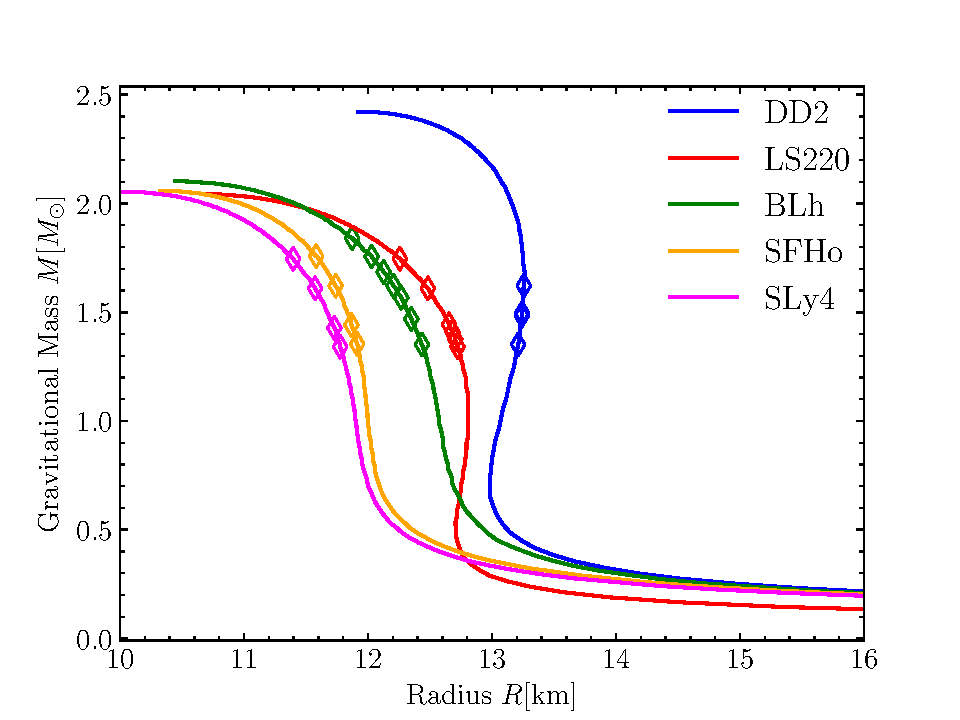
\includegraphics[width=0.49\textwidth]{tov_mr.pdf}
    \caption{Mass-radius relations for the EOSs used in this work. 
        Markers along the sequences indicate the NSs smulated in this work.}  
    \label{fig:method:tov_mr}
\end{figure}

For our models we employ $5$ finite-temperature, composition-dependent equations of state, namely the 
HS(DD2) (hereafter DD2) \cite{Typel:2009sy,Hempel:2009mc}, 
BLh, \cite{Bombaci:2018ksa}, 
LS220, \cite{Lattimer:1991nc}, 
HS(SFHo), (hereafter SFHo) \cite{Steiner:2012rk} and 
SLy4-SOR EOS (hereafter SLy4) \cite{daSilvaSchneider:2017jpg}.

All EOS include neutrinos $(n)$, protons $(p)$, nuclei, electrons, positrons, and photons
as important thermodynamic degrees of freedom.

The radii and maximum masses of neutron stars composed of the cold, neutrino-less $\beta$-equilibrium matter,
from these EOS, fall in line with the current astrophysical constraints, 
\textit{e.g.,} LIGO/Virgo constrain on tidal deformability 
\citep{TheLIGOScientific:2017qsa,Abbott:2018wiz,De:2018uhw,Abbott:2018exr}

All EOS models have symmetry energy at saturation density that are in argeement with experimental limits.
Notably, the LS220 has a especially steep dependency of its symmetry energy on density (\textit{e.g.,} \cite{Lattimer:2012xj,Danielewicz:2013upa}. Thus, this EOS might predict too low symmetry energy below the saturation density. 

%% LS220
The LS220 EOS is based on a non-relativistic (liquid droplet) Skyrme model.
The absolute value of the nuclear bulk incompressibility is set to $220$~MeV, hence, the name.
The EOS includes surface effects and it models $\alpha$-particles as an ideal, classical
non-relativistic gas. For heavy nuclei, the single nucleus approximation is sued. 
%Thus, the the compressible, liquid-drop model with surface effects and composed of ideal gas of 
%particles and heavy nuclei is used to represent the non-homogeneous nuclear matter.
%Heavy nuclei are considered with single nucleus approximation. 
The Gibbs construction is used to model the transition between homogeneous and non-homogeneous matter.
LS220 does not satisfy the constraints from Chiral effective field theory \cite{Hempel:2017ikt}

%% DD2
DD2 (and SFHo) employs the statistical equilibrium to treat the ensemble of several thousands nuclei.
The high-density nuclear matter is treated via RMF approach for unbound nucleons \cite{Hempel:2009mc}.
The excluded volume mechanism is utilized for the phase transition from nuclei to homogeneous
nuclear matter (when densities approch the nuclear saturation density).
DD2 employs the linear, but density dependent coupling for modeling the mean-field nuclear interactions \cite{Typel:2009sy}.
It was however noted that DD2 is not in very good agreement with the so-called flow-constraint \cite{Danielewicz:2002pu}.

%% SFHo [more rephrasing needed!]
Similar to DD2, SFHo combines a statistical ensemble of numerous nuclei, under the assumption of nuclear
statistical equilibrium (NSE) to treat the homogeneous matter, 
with the relativistic mean field approach for the unbound nucleons to treat high-density homogeneous nuclear matter.
It however employs a different parameterizations and values for modeling the mean-field nuclear interactions, 
which is motivated by neutron star radius measurements from low-mass X-ray
binaries (\cite{Steiner:2012rk} and references therein).

The DD2 and SFHo are based on nuclear statistical equilibrium, but 
different parameterizations of the covariant Lagrangian which models the mean-field nuclear interactions.
In these EOSs a finite volume correction coupled to a relativistic mean field theory for treating high-density nuclear matte. However, between these EOSs mean-field nuclear interactions have different parameterizations and values.

%% SLy4
The SLy4 EOS eomplyed in this work is the finite temperature extension \cite{daSilvaSchneider:2017jpg}
of the basic SLY4 Skryme parametrisation for cold nuclear NS matter \cite{Douchin:2001sv}.
The extension includes the non-local isospin asymmetric terms as well as more sophisticated 
treatment of nuclear surface properties and consistent treatment of heavy nuclei size. 
Which is a more advanced version of LS220 treatment (model).
When the phase transition, between the uniform and non-uniform phases, occurs, the phase with lowest 
free energy is chosen, (first order transition).

%% BLh
BLh is a new finite temperature EOS \cite{Logoteta:2020yxf}
This EOS is a finite temperature extension of the cold, $\beta$-equilibrium EOS, \cite{Bombaci:2018ksa},
which was applied to model the BNS merger in \cite{Endrizzi:2018uwl}.
The equation of state is derived in the framework of non-relativistic Brueckner-Hartree-Fock approach.
where microphysical approach based on a specific nuclear interaction is employed for the homogeneous nuclear phase.
The interactions between nucleos are described through a potential derived perturbatively 
in Chiral-Effective-Field theory \cite{Machleidt:2011zz}
The two body interactions are modeled up to second (from the leading term) order, that are used to calculate the local potential. This potential includes $\Delta$-resonances possible excitation. 
Further, the potential is augmented with the three-nucleon force, with the addition of $\Delta$-excitations.
The three-nucleon force was calibrated to reproduce the symmetric nuclear matter at saturatuin density \cite{Logoteta:2016nzc}.
The non-homogeneous phase of the EOS is treated by smoothly connecting the high density BLh EOS to the low-density oart of the SFHo EOS.


\subsubsection{Finite temperature treatment}


Thermal effects are included a different way in these EOS. 
In particular particle correlations beyond the mean field approximation are included only in the BLh EOS.
In other EOS thermal effects enter in the nucleon effective mass, that depend on temperature and density.
These effects, however, are important for the thermal evolution of the NS matter.

%% LS220 and SLy4
In the EOSs that are based on the Skyrme effecrive nuclear interatcions, \textit{e.g.,} LS220 and SLy4
the thermal effects are added in the following form. 
Consider a zero temperature internal energy functional, which depends explicitly on the nuclear density.
The part of this functional that is resposible for interactions is divided into the 
subpart that represents the two-body nucleon-nucleon interactions, (it is quadratic in nuclear density) and a 
subpart that mimics the effect of many body nuclear forces (proportional to the nuclear density in certain power).
Then, both the single particle potentials as well as kinetic energy effective mass dependence play a role
in the temperature dependence of the nuclear effective interaction.
The single particle potential are computed via the variation of the internal energy with respect to the 
neutron and proton densities.
Thus, the smaller the effective masss the larger are kinetic energies and hence, hgiher matter temperature. 
If the entropy remains unchainched.
Thus, the finite temperature behavior of these EOSs is largely set by the nucleon effective mass.
%Then, the smaller the effective mass, the higher the temperature (assuming that entropy is unchanged).
For LS220, the nucleon mass is its bare nucleon mass (for any densities) \gray{so... $m_{N}^*=m_{N}$??}.
For SFHo, $m_N ^* / m_N = 0.76$ at saturation density. 
For DD2 $m_N^*/m_N = 0.56$ 
For BLh $\red{None}$ 
For SLy4 $m_N^*/m_N=0.70$ at saturation density. 
where $m_{N}^*$ is the effective nucleon mass and $m_N$ is the bare nucleon mass.

%% SFHo (and DD2??)
For the SFHo and DD2 EOS, the relativistic Lagrangian considers the $\sigma-$, $\omega-$ and $\rho-$
meson exchanges for descibing nuclear interactions, and the mean-field approximation is used
to solve the resulted Euler-Largrange equations. 
The thermal effects for various species are introduced via Fermi-Dirac distributions at finite temperatures.
Then, self consitent solution of the mean filed eqution introduces the temperature dependence into other 
thermodynamic quantities (through fiurst mesons and nucleon fields)

%% BLh
The BLh EOS employs a different approach to incorporate temperature effects.
The method is based on evaluating the free energy in the Brueckner-Hartree-Fock, which in turn requires,
the effective in-medium nuclear interactions to be defined (starting from the bare nuclear potential).
\gray{This effective interaction is obtained by solving
    the Bethe-Goldstone integral equation which describe the nucleon 
    scattering in the nuclear medium and properly takes into
    account the Pauli principle}.
Then, the nucleon single particle potentials are evaluated (via integration of the on-shell effective interaction matrix)
, which represent the mean field that a nucleon with a certain momenum experience surrounded by other nucleons.
The nucleon single particle potentials, then, allow to evaulate the free energy, and subsequently, 
other thermodynamic quantities.
Notable difference with other EOS discussed here is that the many-body correlations extend beyond the mean field approximation, and are not present in other EOS. 
This EOS was first employed for the BNS merger simulations in \cite{Bernuzzi:2020txg}.

\subsubsection{TOV}

To characterize these EOS, that employs very different microphyscis and finite temperature properties and their relation to the electron fraction, we consider the TOV solutions, presented on the figure \ref{fig:method:tov_mr}.
The maximum mass of a non-rotating NS that these EOSs support are $2.06$, $2.06$, $2.42$ $None$ $None$ 
for SFHo, LS220, DD2, BLh and SLy4 respectively. The NS radii, $R_{1.4}$, then $11.9$, $12.7$, $13.2$ $\red{None}$ $\red{None}$, which in turn is related to the pressure at half saturation density \cite{Lattimer:2012nd}. Thus we adopt the following naming convention for EOS. Those that lead to a NS with smaller radii are called "softer" and those that lead to a NS with larger radii are referred to as "stiffer" EOS.
Among considered, the DD2 is the stiffest EOS, while SLy4 is the softest.